% Options for packages loaded elsewhere
\PassOptionsToPackage{unicode}{hyperref}
\PassOptionsToPackage{hyphens}{url}
%
\documentclass[
]{book}
\usepackage{lmodern}
\usepackage{amssymb,amsmath}
\usepackage{ifxetex,ifluatex}
\ifnum 0\ifxetex 1\fi\ifluatex 1\fi=0 % if pdftex
  \usepackage[T1]{fontenc}
  \usepackage[utf8]{inputenc}
  \usepackage{textcomp} % provide euro and other symbols
\else % if luatex or xetex
  \usepackage{unicode-math}
  \defaultfontfeatures{Scale=MatchLowercase}
  \defaultfontfeatures[\rmfamily]{Ligatures=TeX,Scale=1}
\fi
% Use upquote if available, for straight quotes in verbatim environments
\IfFileExists{upquote.sty}{\usepackage{upquote}}{}
\IfFileExists{microtype.sty}{% use microtype if available
  \usepackage[]{microtype}
  \UseMicrotypeSet[protrusion]{basicmath} % disable protrusion for tt fonts
}{}
\makeatletter
\@ifundefined{KOMAClassName}{% if non-KOMA class
  \IfFileExists{parskip.sty}{%
    \usepackage{parskip}
  }{% else
    \setlength{\parindent}{0pt}
    \setlength{\parskip}{6pt plus 2pt minus 1pt}}
}{% if KOMA class
  \KOMAoptions{parskip=half}}
\makeatother
\usepackage{xcolor}
\IfFileExists{xurl.sty}{\usepackage{xurl}}{} % add URL line breaks if available
\IfFileExists{bookmark.sty}{\usepackage{bookmark}}{\usepackage{hyperref}}
\hypersetup{
  pdftitle={Statistical Modelling},
  pdfauthor={Léo Belzile},
  hidelinks,
  pdfcreator={LaTeX via pandoc}}
\urlstyle{same} % disable monospaced font for URLs
\usepackage{color}
\usepackage{fancyvrb}
\newcommand{\VerbBar}{|}
\newcommand{\VERB}{\Verb[commandchars=\\\{\}]}
\DefineVerbatimEnvironment{Highlighting}{Verbatim}{commandchars=\\\{\}}
% Add ',fontsize=\small' for more characters per line
\usepackage{framed}
\definecolor{shadecolor}{RGB}{248,248,248}
\newenvironment{Shaded}{\begin{snugshade}}{\end{snugshade}}
\newcommand{\AlertTok}[1]{\textcolor[rgb]{0.94,0.16,0.16}{#1}}
\newcommand{\AnnotationTok}[1]{\textcolor[rgb]{0.56,0.35,0.01}{\textbf{\textit{#1}}}}
\newcommand{\AttributeTok}[1]{\textcolor[rgb]{0.77,0.63,0.00}{#1}}
\newcommand{\BaseNTok}[1]{\textcolor[rgb]{0.00,0.00,0.81}{#1}}
\newcommand{\BuiltInTok}[1]{#1}
\newcommand{\CharTok}[1]{\textcolor[rgb]{0.31,0.60,0.02}{#1}}
\newcommand{\CommentTok}[1]{\textcolor[rgb]{0.56,0.35,0.01}{\textit{#1}}}
\newcommand{\CommentVarTok}[1]{\textcolor[rgb]{0.56,0.35,0.01}{\textbf{\textit{#1}}}}
\newcommand{\ConstantTok}[1]{\textcolor[rgb]{0.00,0.00,0.00}{#1}}
\newcommand{\ControlFlowTok}[1]{\textcolor[rgb]{0.13,0.29,0.53}{\textbf{#1}}}
\newcommand{\DataTypeTok}[1]{\textcolor[rgb]{0.13,0.29,0.53}{#1}}
\newcommand{\DecValTok}[1]{\textcolor[rgb]{0.00,0.00,0.81}{#1}}
\newcommand{\DocumentationTok}[1]{\textcolor[rgb]{0.56,0.35,0.01}{\textbf{\textit{#1}}}}
\newcommand{\ErrorTok}[1]{\textcolor[rgb]{0.64,0.00,0.00}{\textbf{#1}}}
\newcommand{\ExtensionTok}[1]{#1}
\newcommand{\FloatTok}[1]{\textcolor[rgb]{0.00,0.00,0.81}{#1}}
\newcommand{\FunctionTok}[1]{\textcolor[rgb]{0.00,0.00,0.00}{#1}}
\newcommand{\ImportTok}[1]{#1}
\newcommand{\InformationTok}[1]{\textcolor[rgb]{0.56,0.35,0.01}{\textbf{\textit{#1}}}}
\newcommand{\KeywordTok}[1]{\textcolor[rgb]{0.13,0.29,0.53}{\textbf{#1}}}
\newcommand{\NormalTok}[1]{#1}
\newcommand{\OperatorTok}[1]{\textcolor[rgb]{0.81,0.36,0.00}{\textbf{#1}}}
\newcommand{\OtherTok}[1]{\textcolor[rgb]{0.56,0.35,0.01}{#1}}
\newcommand{\PreprocessorTok}[1]{\textcolor[rgb]{0.56,0.35,0.01}{\textit{#1}}}
\newcommand{\RegionMarkerTok}[1]{#1}
\newcommand{\SpecialCharTok}[1]{\textcolor[rgb]{0.00,0.00,0.00}{#1}}
\newcommand{\SpecialStringTok}[1]{\textcolor[rgb]{0.31,0.60,0.02}{#1}}
\newcommand{\StringTok}[1]{\textcolor[rgb]{0.31,0.60,0.02}{#1}}
\newcommand{\VariableTok}[1]{\textcolor[rgb]{0.00,0.00,0.00}{#1}}
\newcommand{\VerbatimStringTok}[1]{\textcolor[rgb]{0.31,0.60,0.02}{#1}}
\newcommand{\WarningTok}[1]{\textcolor[rgb]{0.56,0.35,0.01}{\textbf{\textit{#1}}}}
\usepackage{longtable,booktabs}
% Correct order of tables after \paragraph or \subparagraph
\usepackage{etoolbox}
\makeatletter
\patchcmd\longtable{\par}{\if@noskipsec\mbox{}\fi\par}{}{}
\makeatother
% Allow footnotes in longtable head/foot
\IfFileExists{footnotehyper.sty}{\usepackage{footnotehyper}}{\usepackage{footnote}}
\makesavenoteenv{longtable}
\usepackage{graphicx,grffile}
\makeatletter
\def\maxwidth{\ifdim\Gin@nat@width>\linewidth\linewidth\else\Gin@nat@width\fi}
\def\maxheight{\ifdim\Gin@nat@height>\textheight\textheight\else\Gin@nat@height\fi}
\makeatother
% Scale images if necessary, so that they will not overflow the page
% margins by default, and it is still possible to overwrite the defaults
% using explicit options in \includegraphics[width, height, ...]{}
\setkeys{Gin}{width=\maxwidth,height=\maxheight,keepaspectratio}
% Set default figure placement to htbp
\makeatletter
\def\fps@figure{htbp}
\makeatother
\setlength{\emergencystretch}{3em} % prevent overfull lines
\providecommand{\tightlist}{%
  \setlength{\itemsep}{0pt}\setlength{\parskip}{0pt}}
\setcounter{secnumdepth}{5}
% \usepackage{amsmath,amssymb,mathtools}
\usepackage{enumerate}
\usepackage{geometry}
\geometry{hmargin=1.2in}
\usepackage[mathscr]{eucal}
\DeclareMathAlphabet{\mathcrl}{U}{rsfs}{m}{n}
\usepackage{utopia}
\DeclareMathAlphabet{\mathcal}{OMS}{cmsy}{m}{n}
\usepackage{booktabs}
\usepackage{amsthm}
\makeatletter
\def\thm@space@setup{%
  \thm@preskip=8pt plus 2pt minus 4pt
  \thm@postskip=\thm@preskip
}
\makeatother

\usepackage{framed,color}
\definecolor{shadecolor}{RGB}{248,248,248}

\renewcommand{\textfraction}{0.05}
\renewcommand{\topfraction}{0.8}
\renewcommand{\bottomfraction}{0.8}
\renewcommand{\floatpagefraction}{0.75}

\let\oldhref\href
\renewcommand{\href}[2]{#2\footnote{\url{#1}}}

\ifxetex
  \usepackage{letltxmacro}
  \setlength{\XeTeXLinkMargin}{1pt}
  \LetLtxMacro\SavedIncludeGraphics\includegraphics
  \def\includegraphics#1#{% #1 catches optional stuff (star/opt. arg.)
    \IncludeGraphicsAux{#1}%
  }%
  \newcommand*{\IncludeGraphicsAux}[2]{%
    \XeTeXLinkBox{%
      \SavedIncludeGraphics#1{#2}%
    }%
  }%
\fi

\makeatletter
\newenvironment{kframe}{%
\medskip{}
\setlength{\fboxsep}{.8em}
 \def\at@end@of@kframe{}%
 \ifinner\ifhmode%
  \def\at@end@of@kframe{\end{minipage}}%
  \begin{minipage}{\columnwidth}%
 \fi\fi%
 \def\FrameCommand##1{\hskip\@totalleftmargin \hskip-\fboxsep
 \colorbox{shadecolor}{##1}\hskip-\fboxsep
     % There is no \\@totalrightmargin, so:
     \hskip-\linewidth \hskip-\@totalleftmargin \hskip\columnwidth}%
 \MakeFramed {\advance\hsize-\width
   \@totalleftmargin\z@ \linewidth\hsize
   \@setminipage}}%
 {\par\unskip\endMakeFramed%
 \at@end@of@kframe}
\makeatother

\makeatletter
\@ifundefined{Shaded}{
}{\renewenvironment{Shaded}{\begin{kframe}}{\end{kframe}}}
\makeatother

\newenvironment{rmdblock}[1]
  {
  \begin{itemize}
  \renewcommand{\labelitemi}{
    \raisebox{-.7\height}[0pt][0pt]{
      {\setkeys{Gin}{width=3em,keepaspectratio}\includegraphics{images/#1}}
    }
  }
  \setlength{\fboxsep}{1em}
  \begin{kframe}
  \item
  }
  {
  \end{kframe}
  \end{itemize}
  }
\newenvironment{rmdnote}
  {\begin{rmdblock}{note}}
  {\end{rmdblock}}
\newenvironment{rmdcaution}
  {\begin{rmdblock}{caution}}
  {\end{rmdblock}}
\newenvironment{rmdimportant}
  {\begin{rmdblock}{important}}
  {\end{rmdblock}}
\newenvironment{rmdtip}
  {\begin{rmdblock}{tip}}
  {\end{rmdblock}}
\newenvironment{rmdwarning}
  {\begin{rmdblock}{warning}}
  {\end{rmdblock}}
\usepackage[]{natbib}
\bibliographystyle{apalike2}

\title{Statistical Modelling}
\author{Léo Belzile}
\date{version of 2020-06-15}

\begin{document}
\maketitle

\let\href\oldhref

{
\setcounter{tocdepth}{1}
\tableofcontents
}
\hypertarget{preliminary-remarks}{%
\chapter*{Preliminary remarks}\label{preliminary-remarks}}
\addcontentsline{toc}{chapter}{Preliminary remarks}

These notes are licensed under a \href{http://creativecommons.org/licenses/by-nc-sa/4.0/}{Creative Commons Attribution-NonCommercial-ShareAlike 4.0 International License}.

While we show how to implement statistical tests and models in \textbf{SAS} in the class note, the \textbf{R} programming language provides a free alternative. Visit \href{https://cran.r-project.org/}{the R-project website} to download the program. The most popular graphical cross-platform front-end is \href{https://www.rstudio.com/products/rstudio/download/}{RStudio Desktop}.

\textbf{R} is an object-oriented interpreted language. It differs from usual programming languages in that it is designed for interactive analyses. Since \textbf{R} is not a conventional programming language, my teaching approach will be learning-by-doing. The benefit of using \emph{Rmarkdown} is that you see the output directly and you can also copy the code.

\newcommand{\bs}[1]{\boldsymbol{#1}}
\newcommand{\Hmat}{\mathbf{H}}
\newcommand{\Mmat}{\mathbf{M}}
\newcommand{\mX}{\mathbf{X}}
\newcommand{\bX}{{\mathbf{X}}}
\newcommand{\bx}{{\mathbf{x}}}
\newcommand{\by}{{\boldsymbol{y}}}
\newcommand{\bY}{{\boldsymbol{Y}}}
\newcommand{\eps}{\varepsilon}
\newcommand{\beps}{\boldsymbol{\varepsilon}}
\newcommand{\bbeta}{\boldsymbol{\beta}}
\newcommand{\hbb}{\hat{\boldsymbol{\beta}}}
\newcommand{\limni}{\lim_{n \ra \infty}}
\newcommand{\Sp}{\mathscr{S}}
\newcommand{\Hy}{\mathscr{H}}
\newcommand{\E}[2][]{{\mathsf E}_{#1}\left(#2\right)}
\newcommand{\Va}[2][]{{\mathsf{Var}_{#1}}\left(#2\right)}
\newcommand{\I}[1]{{\mathbf 1}_{#1}}

You can find several introductions to \textbf{R} online. Have a look at the \href{https://cran.r-project.org/manuals.html}{\textbf{R} manuals} or better at \href{https://cran.r-project.org/other-docs.html}{contributed manuals}. A nice official reference is \href{http://colinfay.me/intro-to-r/index.html}{An introduction to \textbf{R}}.
You may wish to look up the following chapters of the \textbf{R} language definition (\href{http://colinfay.me/r-language-definition/evaluation-of-expressions.html}{Evaluation of expressions} and part of the \href{http://colinfay.me/r-language-definition/objects.html}{\emph{Objects} chapter}).

If you favor online courses, Data Camp offers a \href{https://www.datacamp.com/courses/free-introduction-to-r}{free introduction to R}.

\hypertarget{basics-of-r}{%
\section{\texorpdfstring{Basics of \textbf{R}}{Basics of R}}\label{basics-of-r}}

\hypertarget{help}{%
\subsection{Help}\label{help}}

Help can be accessed via \texttt{help} or simply \texttt{?}, e.g., \texttt{help("Normal")}. \href{https://www.r-project.org/help.html}{See \textbf{R} page about help files}.

\hypertarget{basic-commands}{%
\subsection{Basic commands}\label{basic-commands}}

Basic \textbf{R} commands are fairly intuitive, especially if you want to use \textbf{R} as a calculator.
Elementary functions such as \texttt{sum}, \texttt{min}, \texttt{max}, \texttt{sqrt}, \texttt{log}, \texttt{exp}, etc., are self-explanatory.

Some (unconventional) features of the language:

\begin{itemize}
\tightlist
\item
  \textbf{R} is case sensitive.
\item
  Use \texttt{\textless{}-} for assignments to a variable, and \texttt{=} for matching arguments inside functions
\item
  Indexing in \textbf{R} starts at 1, \textbf{not} 0.
\item
  Most functions in \textbf{R} are vectorized and loops are typically inefficient.
\item
  Integers are obtained by appending \texttt{L} to the number, so \texttt{2L} is an integer and \texttt{2} a double (\texttt{numerical}).
\end{itemize}

Besides integers and doubles, the common types are

\begin{itemize}
\tightlist
\item
  logical (\texttt{TRUE} and \texttt{FALSE});
\item
  null pointers (\texttt{NULL}), which can be assigned to arguments;
\item
  missing values, namely \texttt{NA} or \texttt{NaN}. These can also be obtained a result of invalid mathematical operations such as \texttt{log(-2)}.
\end{itemize}

Beware! In \textbf{R}, invalid calls will often returns \emph{something} rather than an error. It is therefore good practice to check that the output is sensical.

\hypertarget{linear-algebra-in-r}{%
\subsection{\texorpdfstring{Linear algebra in \textbf{R}}{Linear algebra in R}}\label{linear-algebra-in-r}}

\textbf{R} is an object oriented language, and the basic elements in \textbf{R} are (column) vector. Below is a glossary with some useful commands for performing basic manipulation of vectors and matrix operations:

\begin{itemize}
\tightlist
\item
  \texttt{c} concatenates elements to form a vector
\item
  \texttt{cbind} (\texttt{rbind}) binds column (row) vectors
\item
  \texttt{matrix} and \texttt{vector} are constructors
\item
  \texttt{diag} creates a diagonal matrix (by default with ones)
\item
  \texttt{t} is the function for transpose
\item
  \texttt{rep} creates a vector of duplicates, \texttt{seq} a sequence. For integers \(i\), \(j\) with \(i<j\), \texttt{i:j} generates the sequence \(i, i+1, \ldots, j-1, j\).
\end{itemize}

Subsetting is fairly intuitive and general; you can use vectors, logical statements. For example, if \texttt{x} is a vector,
then

\begin{itemize}
\tightlist
\item
  \texttt{x{[}2{]}} returns the second element
\item
  \texttt{x{[}-2{]}} returns all but the second element
\item
  \texttt{x{[}1:5{]}} returns the first five elements
\item
  \texttt{x{[}(length(x)\ -\ 5):length(x){]}} returns the last five elements
\item
  \texttt{x{[}c(1,\ 2,\ 4){]}} returns the first, second and fourth element
\item
  \texttt{x{[}x\ \textgreater{}\ 3{]}} return any element greater than 3. Possibly an empty vector of length zero!
\item
  \texttt{x{[}\ x\ \textless{}\ -2\ \textbar{}\ x\ \textgreater{}\ 2{]}} multiple logical conditions.
\item
  \texttt{which(x\ ==\ max(x))} index of elements satisfying a logical condition.
\end{itemize}

For a matrix \texttt{x}, subsetting now involves dimensions: \texttt{{[}1,2{]}} returns the element in the first row, second column. \texttt{x{[},2{]}} will return all of the rows, but only the second column. For lists, you can use \texttt{{[}{[}} for subsetting by index or the \texttt{\$} sign by names.

\hypertarget{packages}{%
\subsection{Packages}\label{packages}}

The great strength of \textbf{R} comes from its contributed libraries (called packages), which contain functions and datasets provided by third parties. Some of these (\texttt{base}, \texttt{stats}, \texttt{graphics}, etc.) are loaded by default whenever you open a session.

To install a package from CRAN, use \texttt{install.packages("package")}, replacing \texttt{package} by the package name. Once installed, packages can be loaded using \texttt{library(package)}; all the functions in \texttt{package} will be available in the environment.

\begin{rmdcaution}
\begin{rmdcaution}

There are drawbacks to loading packages: if an object with the same name from another package is already present in your environment, it will be hidden. Use the double-colon operator \texttt{::} to access a single object from an installed package (\texttt{package::object}).

\end{rmdcaution}
\end{rmdcaution}

\hypertarget{week1}{%
\section{Tutorial 1}\label{week1}}

\hypertarget{datasets}{%
\subsection{Datasets}\label{datasets}}

\begin{itemize}
\tightlist
\item
  datasets are typically stored inside a \texttt{data.frame}, a matrix-like object whose columns contain the variables and the rows the observation vectors.
\item
  The columns can be of different types (\texttt{integer}, \texttt{double}, \texttt{logical}, \texttt{character}), but all the column vectors must be of the same length.
\item
  Variable names can be displayed by using \texttt{names(faithful)}.
\item
  Individual columns can be accessed using the column name using the \texttt{\$} operator. For example, \texttt{faithful\$eruptions} will return the first column of the \texttt{faithful} dataset.
\item
  To load a dataset from an (installed) \textbf{R} package, use the command \texttt{data} with the name of the \texttt{package} as an argument (must be a string). The package \texttt{datasets} is loaded by default whenever you open \textbf{R}, so these are always in the search path.
\end{itemize}

The following functions can be useful to get a quick glimpse of the data:

\begin{itemize}
\tightlist
\item
  \texttt{summary} provides descriptive statistics for the variable.
\item
  \texttt{str} provides the first few elements with each variable, along with the dimension
\item
  \texttt{head} (\texttt{tail}) prints the first (last) \(n\) lines of the object to the console (default is \(n=6\)).
\end{itemize}

We start by loading a dataset of the Old Faithful Geyser of Yellowstone National park and looking at its entries.

\begin{Shaded}
\begin{Highlighting}[]
\CommentTok{# Load Old faithful dataset}
\KeywordTok{data}\NormalTok{(faithful, }\DataTypeTok{package =} \StringTok{"datasets"}\NormalTok{)}
\CommentTok{# Query the database for documentation}
\NormalTok{?faithful}
\CommentTok{# look at first entries}
\KeywordTok{head}\NormalTok{(faithful)}
\end{Highlighting}
\end{Shaded}

\begin{verbatim}
##   eruptions waiting
## 1       3.6      79
## 2       1.8      54
## 3       3.3      74
## 4       2.3      62
## 5       4.5      85
## 6       2.9      55
\end{verbatim}

\begin{Shaded}
\begin{Highlighting}[]
\KeywordTok{str}\NormalTok{(faithful)}
\end{Highlighting}
\end{Shaded}

\begin{verbatim}
## 'data.frame':    272 obs. of  2 variables:
##  $ eruptions: num  3.6 1.8 3.33 2.28 4.53 ...
##  $ waiting  : num  79 54 74 62 85 55 88 85 51 85 ...
\end{verbatim}

\begin{Shaded}
\begin{Highlighting}[]
\CommentTok{# What kind of object is faithful? }
\KeywordTok{class}\NormalTok{(faithful)}
\end{Highlighting}
\end{Shaded}

\begin{verbatim}
## [1] "data.frame"
\end{verbatim}

Other common classes of objects:

\begin{itemize}
\tightlist
\item
  \texttt{matrix}: an object with attributes \texttt{dim}, \texttt{ncol} and \texttt{nrow} in addition to \texttt{length}, which gives the total number of elements.
\item
  \texttt{array}: a higher dimensional extension of \texttt{matrix} with arguments \texttt{dim} and \texttt{dimnames}.
\item
  \texttt{list}: an unstructured class whose elements are accessed using double indexing \texttt{{[}{[}\ {]}{]}} and elements are typically accessed using \texttt{\$} symbol with names. To delete an element from a list, assign \texttt{NULL} to it.
\item
  \texttt{data.frame} is a special type of list where all the elements are vectors of potentially different type, but of the same length.
\end{itemize}

\hypertarget{graphics}{%
\subsection{Graphics}\label{graphics}}

The \texttt{faithful} dataset consists of two variables: the regressand \texttt{waiting} and the regressor \texttt{eruptions}. One could postulate that the waiting time between eruptions will be smaller if the eruption time is small, since pressure needs to build up for the eruption to happen. We can look at the data to see if there is a linear relationship between the variables.

An image is worth a thousand words and in statistics, visualization is crucial. Scatterplots are produced using the function \texttt{plot}. You can control the graphic console options using \texttt{par} --- see \texttt{?plot} and \texttt{?par} for a description of the basic and advanced options available.

Once \texttt{plot} has been called, you can add additional observations as points (lines) to the graph using \texttt{point} (\texttt{lines}) in place of \texttt{plot}. If you want to add a line (horizontal, vertical, or with known intercept and slope), use the function \texttt{abline}.

Other functions worth mentioning at this stage:

\begin{itemize}
\tightlist
\item
  \texttt{boxplot} creates a box-and-whiskers plot
\item
  \texttt{hist} creates an histogram, either on frequency or probability scale (option \texttt{freq\ =\ FALSE}). \texttt{breaks} control the number of bins. \texttt{rug} adds lines below the graph indicating the value of the observations.
\item
  \texttt{pairs} creates a matrix of scatterplots, akin to \texttt{plot} for data frame objects.
\end{itemize}

\begin{rmdnote}
\begin{rmdnote}

There are two options for basic graphics: the base graphics package and the package \texttt{ggplot2}. The latter is a more recent proposal that builds on a modular approach and is more easily customizable --- I suggest you stick to either and \texttt{ggplot2} is a good option if you don't know \textbf{R} already, as the learning curve will be about the same. Even if the display from \texttt{ggplot2} is nicer, this is no excuse for not making proper graphics. Always label the axis and include measurement units!

\end{rmdnote}
\end{rmdnote}

\hypertarget{introduction}{%
\chapter{Introduction}\label{introduction}}

The goal of this course is to introduce the fundamental principles of statistical \emph{inference} as well as advanced statistical methods used in business intelligence problems. We will also see applications of these methods using (mostly) simulated and real data applications using dedicated software. The \textbf{SAS} material is presented throughout the course slides, whereas \textbf{R} will be presented in this online book.

This introductory chapter touches many topics that may be covered in undergraduate statistics courses, including notions about hypothesis test (null and alternative hypothesis, statistics, null distributions, levels and power of test, confidence interval).

This chapter also includes a short description of population and samples, basic graphics (scatterplot, violinplots, histograms, box-and-whisker plots) and tests for one-sample location problems (signed test, signed rank test and one-sample and paired \emph{t}-tests). Recommended reading are Chapter 1--4 of the OpenIntro book \href{https://www.openintro.org/stat/textbook.php?stat_book=isrs}{``Introductory Statistics with
Randomization and Simulation''}.

\hypertarget{statistical-inference-versus-predictions}{%
\section{Statistical inference versus predictions}\label{statistical-inference-versus-predictions}}

Statistical inference deals with explanatory models --- used for answering scientific questions, i.e.~test research hypotheses concerning variable effects. However, these models can also be used to make predictions.

\hypertarget{reminders-and-objectives}{%
\section{Reminders and Objectives}\label{reminders-and-objectives}}

This section covers some basics about population and samples, hypothesis tests and duality between confidence intervals and \(p\)-values.

\hypertarget{population-and-sample}{%
\section{Population and sample}\label{population-and-sample}}

Statistics is about drawing inference from a large group given a representative subset of limited size; we cannot measure for practical and financial reasons a characteristic such as height to get the average length of a human. Often, it is also unnecessary: conclusions drawn from a sample are good enough.

The \textbf{population} is the target group under study. A \textbf{sample} is a representative subset of the population for which we measure a characteristic. For example, if we are interested in voting intentions for the next federal election, the population would consist of all Canadian citizens aged 18 or more at the day the vote takes place. Pollsters may select a small group of eligible voters and ask them for their voting preferences: you can get pretty good estimates even when 17.5 millions people vote, as the margin of error of a probabilistic sample with 1000 participants is about 3\% with 95\% confidence level.

The population is often defined in the context of a study, but one should be careful in not making this definition too narrow. If you want to do a study of breast cancer, you do not want to define the population to be all patients at a given hospital who received a diagnostic of breast cancer; rather, you should aim to have a broad enough definition so that you can generalize your results.
Choosing a sample is hard, and an entire branch of statistics, survey sampling, deals specifically with this. For opinion polls, pollster often have polls and databases of phone numbers to pick from. What makes it more challenging nowadays is that a large share of individuals do not own a landline anymore (and so their phone number is not public), but calling only cellphones leads to bias because it undersample elderly people; selecting exclusively one or the other leads to bad samples.

\hypertarget{testing-statistical-hypotheses}{%
\section{Testing statistical hypotheses}\label{testing-statistical-hypotheses}}

Hypothesis testing is ubiquitous in statistics, yet often poorly understood. The topic is thus presented in an intuitive manner through examples by making an analogy with trial for murder. We review the formulation of null and alternative hypotheses, the choice of test statistic, derivation of its null distribution and finally conclusions in light of \(p\)-value. As an illustrative example, we test for equal means for two groups using a permutation test.

The best analogy I have for hypothesis testing is a criminal trial: you are a jury member for a murder case and are asked to deliver a verdict, which will be either \emph{guilty} or \emph{not guilty}, based on evidence presented in court. By default, the presumption of innocence apply so your default position is that the accused is not guilty and you analyze evidences in this optic to avoid judicial errors (do not condemn an innocent to death). Only if the evidences presented by the prosecutor are overwhelming will you declare the person \emph{guilty}.

We can make a parallel with hypothesis testing as follows:

\begin{itemize}
\tightlist
\item
  there are only two possible options considered, which correspond to the null hypothesis \(H_0\) (the accused is innocent of the murder) and the alternative \(H_1\) (the accused committed the murder).
\item
  the test statistic comprises all evidences. There are many different choices, but not all of them are good (compare DNA samples with circumstantial evidences).
\item
  rejecting the null hypothesis corresponds to the \emph{guilty} verdict, i.e., reject \(H_0\).
\item
  sometimes, there are plenty of evidences presented even when the individual accused of murder is innocent. To minimize the risk of judicial error, we only reject if these are overwhelming, meaning that the probability of happening by chance for an innocent are equal to some tolerance level \(\alpha\), specified beforehand. The \textbf{level of a test} does not change.
\item
  if we fail to reject the null hypothesis, corresponding to a verdict of \emph{not guilty}, this means either of two things: the person is innocent or we have a reasonable doubt. The jury only weights the evidence in light of the apriori assumption that the accused is innocent unless proven otherwise, so we cannot conclude anything about innocence.
\item
  our ability to correctly declare a murderer guilty is called \emph{power}. The choice of test statistic (evidences) determines how well we can confound murdererers. Power is a probability: the higher, the better. A test with no power is useless. If you have to choose a single evidence from the proof, you might select `blood stains on the accused's clothes which matches the DNA victim' over `he happened to be in the city as the victim when the murder was committed'.
\end{itemize}

The interplay between Type I and Type II errors are best displayed graphically. Nathaniel Stevens (University of Waterloo) made a nice \href{https://nathaniel-t-stevens.shinyapps.io/ErrorIllustrator/}{Shiny app}.
In these plots, \(\alpha\) is the significance level (usually 5\%) corresponding to the type I error we are willing to commit. The effect size measures the difference between the null hypothesis and the true effect size (think about measuring height of people in two populations, with the null hypothesis being that there is no difference). If there was truly a difference, but the latter was small, say 0.01cm, it would be confounded with the measurement variability. On the other hand, if the true difference is 10cm, it would be pretty obvious.
The main factors affecting power are sample size and variability in the population; the variability of the mean estimate goes down like \(\sigma/\sqrt{n}\), so decreases when either (a) \(\sigma\) decreases or (b) \(n\) increases. With large enough samples, all differences will be detected. The type I error is the surface represented in red (\(\alpha\)), whereas the type II error (false negative) is \(\beta\) in blue. The power is the area of the density in dashed blue; the larger, the more the test is capable of detecting when the null hypothesis is false.

\hypertarget{exploratory-data-analysis}{%
\section{Exploratory data analysis}\label{exploratory-data-analysis}}

Looking at the data is arguably the most important of an analysis. This step consists in looking at summary statistics (mean, quantiles, min and max) and to plot the data, one variable at a time and then pairs. This will allow you to detect outliers (for example, missing values were often encoded with \(-1\) or \(999\) in the old days when only numerical values could be saved by devices). Real data is messy, and often artefacts (e.g., rounding, ties) are most easily viewed from scatterplot, histograms, box-and-whiskers plots, etc.

\begin{itemize}
\tightlist
\item
  a box-and-whiskers plot (or boxplot), consists of a box composed by the 25, 50 and 75 percentiles. The median separates the box, while the whiskers extend beyond 1.5 times the interquartile range (the length of the box). Values that fall outside of this range are often represented by dots and would be extreme points, if the sample was normally distributed.
\item
  a histogram bins observations and can be useful to detect outliers and multimodality. The number of bins is often selected automatically.
\item
  a kernel density estimator represents local fit of the density function and is a continuous analog of the histogram if the latter is on the density scale (as opposed to frequency). The kernel density is more sensitive to local deviations and may more easily capture discreteness. The bandwidth controls the amount of neighboring data used for the fit. Optimal (and default) choices are typically selected.
\end{itemize}

\hypertarget{one-sample-and-two-sample-location-tests}{%
\chapter{One-sample and two-sample location tests}\label{one-sample-and-two-sample-location-tests}}

\hypertarget{one-sample-and-paired-t-test}{%
\section{\texorpdfstring{One-sample and paired \emph{t}-test}{One-sample and paired t-test}}\label{one-sample-and-paired-t-test}}

We covered this example of Tech3Lab comparing the reaction time between individuals for two tasks, texting and speaking on the phone, while walking. The response variable is reaction time in seconds to the presence of a bicycle moving towards the participant.

The data can be found in \texttt{distraction.txt} and can be loaded in \textbf{R} in a \texttt{data.frame} object.

\begin{Shaded}
\begin{Highlighting}[]
\CommentTok{# get URL of the file}
\NormalTok{url <-}\StringTok{ "https://lbelzile.bitbucket.io/MATH60619A/distraction.txt"}
\CommentTok{# load data, stating header}
\NormalTok{data <-}\StringTok{ }\KeywordTok{read.table}\NormalTok{(url, }\DataTypeTok{header =} \OtherTok{TRUE}\NormalTok{)}
\end{Highlighting}
\end{Shaded}

The columns of a \texttt{data.frame} object can be accessed using the \texttt{\$} operator.

We can calculate descriptive statistics for the data by using the commands \texttt{summary}, or \texttt{mean}, \texttt{sd}, etc.

Our goal is to compare the average reaction time for texting \texttt{t} and for call \texttt{c}, say \(\mu_C=\mu_T\). Since the individuals complete the two assignments (the order is random), we are looking at a paired \(t\)-test, which amounts to comparing the null \(\mathscr{H}_0: \mu_D=0\), where \(\mu_D\) is the difference (in seconds) between the reaction time for texting vs phone conversation in the population. We can assess this graphically through an histogram of the distribution.

\begin{Shaded}
\begin{Highlighting}[]
\CommentTok{# create new vector as difference in time}
\NormalTok{D <-}\StringTok{ }\NormalTok{data}\OperatorTok{$}\NormalTok{t }\OperatorTok{-}\StringTok{ }\NormalTok{data}\OperatorTok{$}\NormalTok{c}
\CommentTok{# histogram, on the probability scale}
\KeywordTok{hist}\NormalTok{(D, }\DataTypeTok{probability =} \OtherTok{TRUE}\NormalTok{, }
     \DataTypeTok{xlab =} \StringTok{"Time difference between reaction time}
\StringTok{         for texting and call (in seconds)"}\NormalTok{,}
     \DataTypeTok{main =} \StringTok{""}\NormalTok{)}
\CommentTok{# add density estimate}
\KeywordTok{lines}\NormalTok{(}\KeywordTok{density}\NormalTok{(D))}
\end{Highlighting}
\end{Shaded}

\begin{center}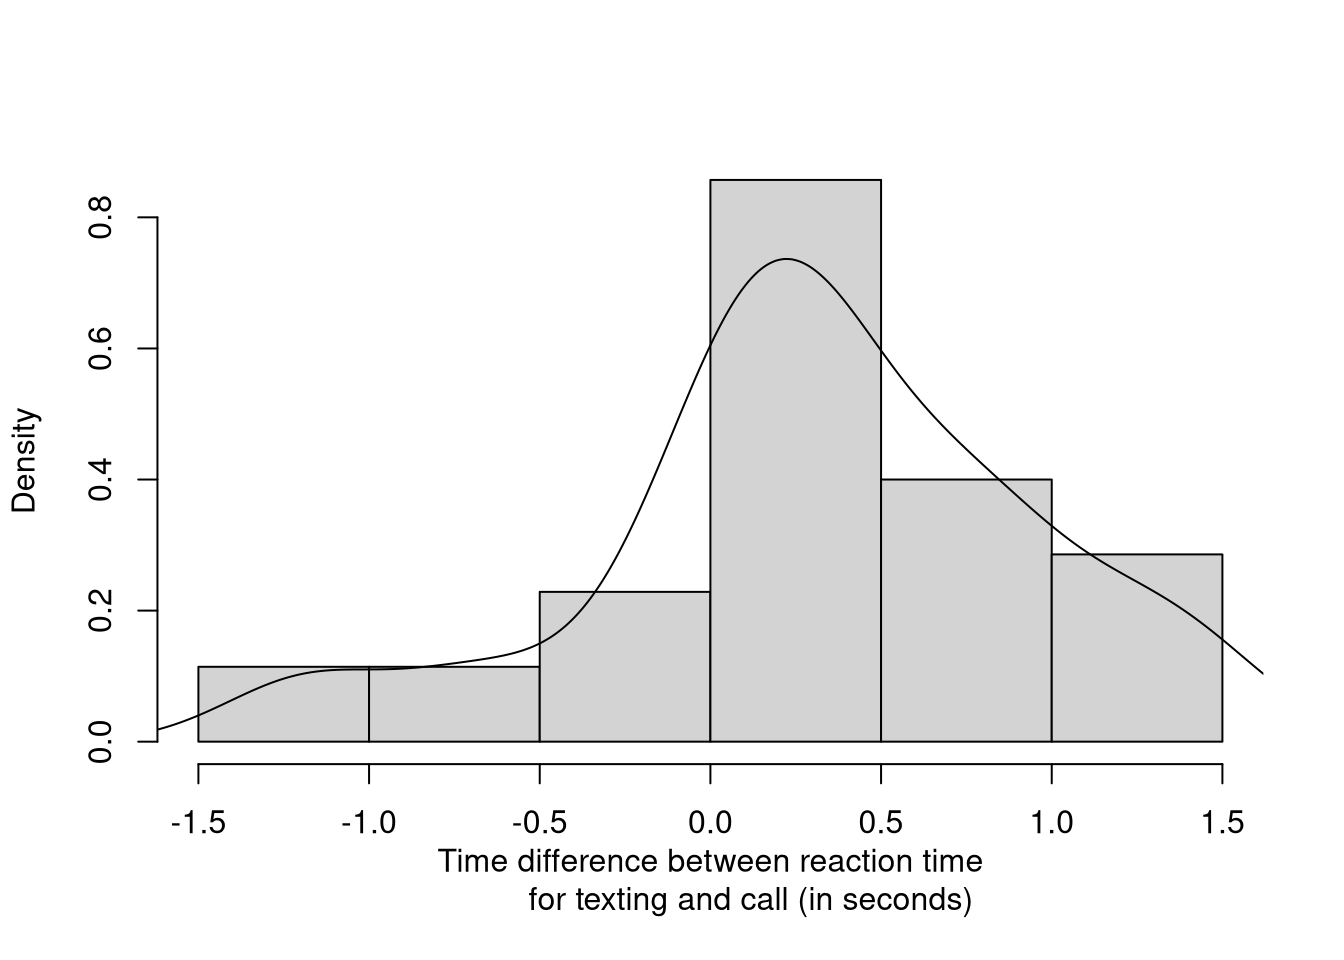
\includegraphics[width=0.7\linewidth]{Statistical-modelling_files/figure-latex/hist_distract-1} \end{center}

The two sample mean (standard error) are different, 1.39 (0.53) seconds for texting and 1.08 (0.4) seconds for call. To check if this is really the case, we perform a paired \(t\)-test.

\begin{Shaded}
\begin{Highlighting}[]
\NormalTok{ttest <-}\StringTok{ }\KeywordTok{t.test}\NormalTok{(}\DataTypeTok{x =}\NormalTok{ data}\OperatorTok{$}\NormalTok{t, }\DataTypeTok{y =}\NormalTok{ data}\OperatorTok{$}\NormalTok{c, }
                \DataTypeTok{alternative =} \StringTok{"two.sided"}\NormalTok{, }\DataTypeTok{paired =} \OtherTok{TRUE}\NormalTok{)}
\KeywordTok{print}\NormalTok{(ttest)}
\end{Highlighting}
\end{Shaded}

\begin{verbatim}
## 
##  Paired t-test
## 
## data:  data$t and data$c
## t = 3, df = 34, p-value = 0.006
## alternative hypothesis: true difference in means is not equal to 0
## 95 percent confidence interval:
##  0.094 0.532
## sample estimates:
## mean of the differences 
##                    0.31
\end{verbatim}

The output provides the value of the test statistic \(t = \overline{D}/\mathsf{se}(\overline{D})=\) 2.91 with associated \(p\)-value . We strongly reject the null hypothesis that \(\mu_C=\mu_D\) at level 5\% (even 1\%), meaning that the reaction time is significantly longer on average for texting with an estimated 95\% confidence of \([\) 0.09, 0.53 \(]\).

The null distribution of the test statistic is \(\mathcal{T}_{34}\), so we can look at how extreme our test statistic is relative to a typical value from the null distribution.

\begin{center}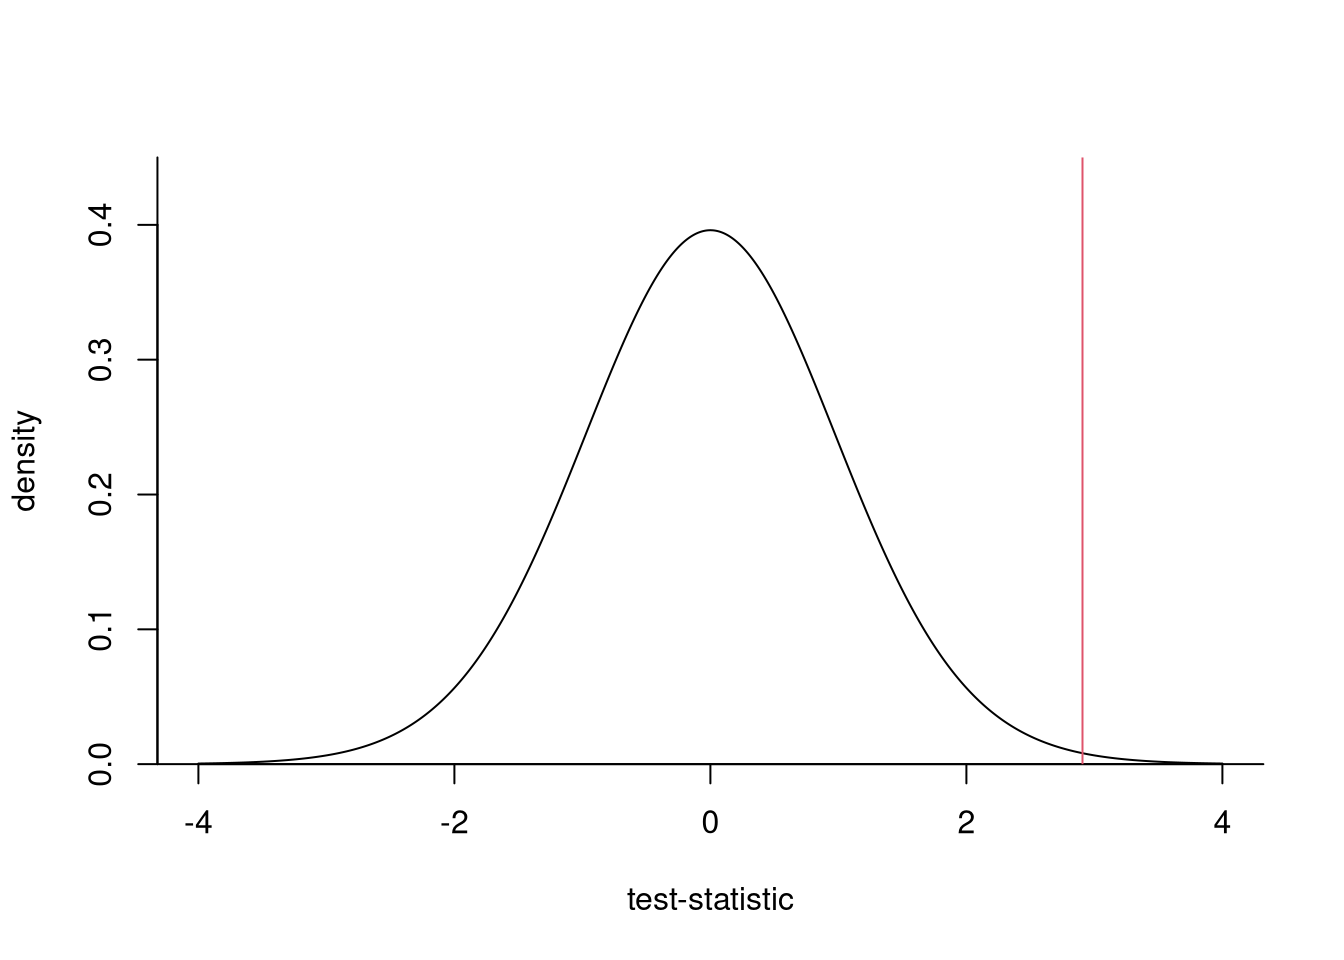
\includegraphics[width=0.7\linewidth]{Statistical-modelling_files/figure-latex/tdensity-1} \end{center}

We can also do a one-sample \(t\)-test using the same function. The \texttt{hours} dataset consists of a sample of size \(n=100\) of workers who had attained at least a college degree. We could test whether the participants work 40 hours a week (two sided alternative), or if they work more than that. In the latter case, the null hypothesis is thus \(\mathscr{H}_0: \mu \geq 40\), where \(\mu\) is the average number of weekly work hours, against the alternative \(\mathscr{H}_1: \mu < 40\).

\begin{Shaded}
\begin{Highlighting}[]
\NormalTok{url <-}\StringTok{ "https://lbelzile.bitbucket.io/MATH60619A/hours.txt"}
\NormalTok{data <-}\StringTok{ }\KeywordTok{read.table}\NormalTok{(}\DataTypeTok{file =}\NormalTok{ url, }\DataTypeTok{header =} \OtherTok{TRUE}\NormalTok{)}
\NormalTok{ttest_twosided <-}\StringTok{ }\KeywordTok{t.test}\NormalTok{(data, }\DataTypeTok{alternative =} \StringTok{"two.sided"}\NormalTok{, }\DataTypeTok{mu =} \DecValTok{40}\NormalTok{)}
\NormalTok{ttest_onesided <-}\StringTok{ }\KeywordTok{t.test}\NormalTok{(data, }\DataTypeTok{alternative =} \StringTok{"greater"}\NormalTok{, }\DataTypeTok{mu =} \DecValTok{40}\NormalTok{)}
\end{Highlighting}
\end{Shaded}

In both cases, we reject the null hypothesis at level 5\%, but the one-sided alternative has a smaller \(p\)-value. Think about why it does not make sense to test for \(\mathscr{H}_0: \mu \leq 40\) versus \(\mathscr{H}_1: \mu >40\) in view of the sample mean.

\hypertarget{two-sample-t-test}{%
\section{\texorpdfstring{Two-sample \emph{t}-test}{Two-sample t-test}}\label{two-sample-t-test}}

We use the same example covered in slides for the \texttt{tickets} data. Since the research question is ``Does paying by credit card encourage consumers to pay more?'', this calls for a one sided test, with \(\mathscr{H}_1: \mu_{\text{cred}} > \mu_{\text{cash}}\) and \emph{de facto} the null hypothesis must be \(\mathscr{H}_0: \mu_{\text{cred}} \leq \mu_{\text{cash}}\). The alternative hypothesis is the one we \emph{would} be interested in checking, but because we are the Devil's advocate, the null hypothesis is the opposite and includes all other possibilities. Note that we only need to consider the case \(\mu_{\text{cred}} = \mu_{\text{cash}}\) (why?), so one often write this as the null hypothesis.

We can start by loading the data and preliminary visual inspection. In light of the boxplot, it seems that the variance in the two groups differs.

\begin{Shaded}
\begin{Highlighting}[]
\NormalTok{url <-}\StringTok{ "https://lbelzile.bitbucket.io/MATH60619A/tickets.txt"}
\NormalTok{tickets <-}\StringTok{ }\KeywordTok{read.table}\NormalTok{(url, }\DataTypeTok{header =} \OtherTok{TRUE}\NormalTok{) }\CommentTok{#load data}
\KeywordTok{head}\NormalTok{(tickets) }\CommentTok{#print first six lines}
\end{Highlighting}
\end{Shaded}

\begin{verbatim}
##   offer group
## 1    62  cash
## 2    44  cash
## 3    46  cash
## 4    48  cash
## 5    50  cash
## 6    58  cash
\end{verbatim}

\begin{Shaded}
\begin{Highlighting}[]
\KeywordTok{boxplot}\NormalTok{(offer }\OperatorTok{~}\StringTok{ }\NormalTok{group, }\DataTypeTok{data =}\NormalTok{ tickets)}
\end{Highlighting}
\end{Shaded}

\begin{center}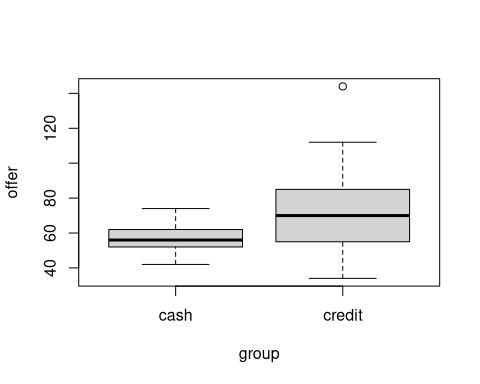
\includegraphics[width=0.7\linewidth]{Statistical-modelling_files/figure-latex/loadtickets-1} \end{center}

\begin{Shaded}
\begin{Highlighting}[]
\NormalTok{tickets}\OperatorTok{$}\NormalTok{group <-}\StringTok{ }\KeywordTok{factor}\NormalTok{(}\DataTypeTok{x =}\NormalTok{ tickets}\OperatorTok{$}\NormalTok{group, }\CommentTok{#cast binary to categ}
                        \DataTypeTok{labels =} \KeywordTok{c}\NormalTok{(}\StringTok{"cash"}\NormalTok{,}\StringTok{"credit"}\NormalTok{)) }\CommentTok{#assign meaningful }
\CommentTok{# summarize data by group (equivalent of PROC MEANS in SAS)}
\KeywordTok{with}\NormalTok{(}\DataTypeTok{data =}\NormalTok{ tickets, }\CommentTok{#use data}
     \DataTypeTok{expr =} \KeywordTok{by}\NormalTok{(}\DataTypeTok{data =}\NormalTok{ offer, }\DataTypeTok{FUN =}\NormalTok{ summary, }\DataTypeTok{INDICES =}\NormalTok{ group))}
\end{Highlighting}
\end{Shaded}

\begin{verbatim}
## group: cash
##    Min. 1st Qu.  Median    Mean 3rd Qu.    Max. 
##      42      52      56      57      62      74 
## ------------------------------------------------------------ 
## group: credit
##    Min. 1st Qu.  Median    Mean 3rd Qu.    Max. 
##      34      55      70      72      85     144
\end{verbatim}

\begin{Shaded}
\begin{Highlighting}[]
\KeywordTok{with}\NormalTok{(}\DataTypeTok{data =}\NormalTok{ tickets, }
     \DataTypeTok{expr =} \KeywordTok{by}\NormalTok{(}\DataTypeTok{data =}\NormalTok{ offer, }\DataTypeTok{FUN =}\NormalTok{ sd, }\DataTypeTok{INDICES =}\NormalTok{ group))}
\end{Highlighting}
\end{Shaded}

\begin{verbatim}
## group: cash
## [1] 7.5
## ------------------------------------------------------------ 
## group: credit
## [1] 24
\end{verbatim}

\begin{Shaded}
\begin{Highlighting}[]
\CommentTok{# alternatively}
\CommentTok{# sd(tickets$offer[tickets$group == "cash"])}
\end{Highlighting}
\end{Shaded}

The option \texttt{header\ =\ TRUE} specifies that the first line of the file contains the name of the variables. While \texttt{read.table} is the default for command to read tables (with options \texttt{sep} for the separator, we will also encounter \texttt{read.csv} for comma-separated values. The data is stored in a \texttt{data.frame} object. The command \texttt{str} gives a description of the observations (with the type) and \texttt{head} prints the first lines. Other relevant commands include \texttt{ndim}, \texttt{nrow} and \texttt{ncol} that give the dimensions of the data, the number of rows and the number of columns, respectively.

Reference to the columns of a data frame is made using their column names (\texttt{colnames(tickets)}) using \texttt{\$}, so \texttt{tickets\$group} returns the second column with the binary variable. Alternatively, we can use the \texttt{attach} command to attach the dataset, in which case the variables are now accessible directly. Beware with this, as there is a risk of having multiple objects with the same name. A good practice is to \texttt{detach} the dataset after use.

When we load a dataset, the default option for strings is to cast them to factor (i.e., categorical variables). We do this likewise for the binary variables, even if in this case this makes no difference (but it is good practice).

Summary statistics showed that the mean amount offered for tickets is 56.61 (7.5) for the group paying by cash and 71.61 (23.6), but we need to perform a test in order to know whether such a difference, -15.01, is significative. Since our null hypothesis is that customers are willing to pay more by credit card, we perform a one-sided \(t\)-test.

\begin{Shaded}
\begin{Highlighting}[]
\NormalTok{ttest <-}\StringTok{ }\KeywordTok{t.test}\NormalTok{(}\DataTypeTok{formula =}\NormalTok{ offer }\OperatorTok{~}\StringTok{ }\NormalTok{group, }
       \DataTypeTok{data =}\NormalTok{ tickets, }
       \DataTypeTok{alternative =} \StringTok{"less"}\NormalTok{, }\CommentTok{#one-sided}
       \DataTypeTok{var.equal =} \OtherTok{TRUE}\NormalTok{) }\CommentTok{#by default FALSE}
\KeywordTok{print}\NormalTok{(ttest)}
\end{Highlighting}
\end{Shaded}

\begin{verbatim}
## 
##  Two Sample t-test
## 
## data:  offer by group
## t = -3, df = 62, p-value = 0.0005
## alternative hypothesis: true difference in means is less than 0
## 95 percent confidence interval:
##  -Inf -7.8
## sample estimates:
##   mean in group cash mean in group credit 
##                   57                   72
\end{verbatim}

In \textbf{R}, the default option for the function \texttt{t.test} is Welch's test (\texttt{var.equal\ =\ FALSE}), since the latter is valid whether or not the variance of the two groups are equal. The value of the test statistic is -3.48, which should follow a Student \(t\) distribution under \(H_0\) with degrees of freedom, leading to a \(p\)-value smaller than \(10 \times 10^{-3}\). We reject the null at level \(\alpha=0.05\) in favor of the alternative that people paying by credit card are willing to spend more than those paying by cash with the lower bound of the 95\% confidence interval for this difference being -7.8.

The equality test for the variance is not calculated directly by \texttt{t.test} in \textbf{R}, but the function \texttt{var.test} implements an \(F\) test for this hypothesis (Levene's test is in \texttt{car::leveneTest}). We have overwhelming evidence that the variance for the two groups are unequal, so we can should Welch's test rather that the two-sample \(t\)-test. The conclusions are the same in this case, namely that such a difference is implausible if the true average were equal.

\begin{Shaded}
\begin{Highlighting}[]
\KeywordTok{var.test}\NormalTok{(}\DataTypeTok{formula =}\NormalTok{ offer }\OperatorTok{~}\StringTok{ }\NormalTok{group, }
       \DataTypeTok{data =}\NormalTok{ tickets)}
\end{Highlighting}
\end{Shaded}

\begin{verbatim}
## 
##  F test to compare two variances
## 
## data:  offer by group
## F = 0.1, num df = 32, denom df = 30, p-value = 6e-09
## alternative hypothesis: true ratio of variances is not equal to 1
## 95 percent confidence interval:
##  0.05 0.21
## sample estimates:
## ratio of variances 
##                0.1
\end{verbatim}

\begin{Shaded}
\begin{Highlighting}[]
\CommentTok{#Levene's test (same as SAS output)}
\NormalTok{car}\OperatorTok{::}\KeywordTok{leveneTest}\NormalTok{(offer }\OperatorTok{~}\StringTok{ }\NormalTok{group, }
       \DataTypeTok{data =}\NormalTok{ tickets)}
\end{Highlighting}
\end{Shaded}

\begin{verbatim}
## Levene's Test for Homogeneity of Variance (center = median)
##       Df F value  Pr(>F)    
## group  1    16.4 0.00014 ***
##       62                    
## ---
## Signif. codes:  0 '***' 0.001 '**' 0.01 '*' 0.05 '.' 0.1 ' ' 1
\end{verbatim}

\begin{Shaded}
\begin{Highlighting}[]
\KeywordTok{t.test}\NormalTok{(}\DataTypeTok{formula =}\NormalTok{ offer }\OperatorTok{~}\StringTok{ }\NormalTok{group, }
       \DataTypeTok{data =}\NormalTok{ tickets, }
       \DataTypeTok{alternative =} \StringTok{"less"}\NormalTok{)}
\end{Highlighting}
\end{Shaded}

\begin{verbatim}
## 
##  Welch Two Sample t-test
## 
## data:  offer by group
## t = -3, df = 36, p-value = 0.0009
## alternative hypothesis: true difference in means is less than 0
## 95 percent confidence interval:
##  -Inf -7.5
## sample estimates:
##   mean in group cash mean in group credit 
##                   57                   72
\end{verbatim}

It now remains to check the normality assumption graphically; \textbf{SAS} prints histograms with superimposed densities and box-and-whiskers plots. We can also add quantile-quantile plots; the basic function is \texttt{qqnorm} in \textbf{R} and \texttt{qqline} adds a line passing through the first and third quartile, but we use the \texttt{qqPlot} function from the \texttt{car} package instead, since the latter includes a grid in the background and simulated approximate 95\% pointwise confidence intervals. The discreteness of the observations in the cash group is visible (corresponding to horizontal segments). Here, due to large enough sample sizes, we have no evidence against normality even if the variances are obviously different.

\begin{Shaded}
\begin{Highlighting}[]
\KeywordTok{par}\NormalTok{(}\DataTypeTok{mfrow =} \KeywordTok{c}\NormalTok{(}\DecValTok{1}\NormalTok{,}\DecValTok{2}\NormalTok{), }\DataTypeTok{mar =} \KeywordTok{c}\NormalTok{(}\DecValTok{4}\NormalTok{,}\DecValTok{4}\NormalTok{,}\DecValTok{1}\NormalTok{,}\DecValTok{1}\NormalTok{)) }\CommentTok{#change margins,}
\CommentTok{# mfrow = c(1,2) gives two plots side by side}
\KeywordTok{boxplot}\NormalTok{(offer }\OperatorTok{~}\StringTok{ }\NormalTok{group, }\DataTypeTok{data =}\NormalTok{ tickets, }
        \DataTypeTok{main =} \StringTok{"Box-and-whiskers plot"}\NormalTok{, }
        \DataTypeTok{ylab =} \StringTok{"Amount offered (in dollars)"}\NormalTok{,}
        \DataTypeTok{frame =} \OtherTok{FALSE}\NormalTok{)}

\CommentTok{# Histogram }
\CommentTok{# Attach dataset - variables (columns) are now visible}
\CommentTok{# avoids having tickets$group everywhere, now group}
\KeywordTok{attach}\NormalTok{(tickets)}
\KeywordTok{hist}\NormalTok{(}\DataTypeTok{x =}\NormalTok{ offer[group }\OperatorTok{==}\StringTok{ "cash"}\NormalTok{], }
     \DataTypeTok{breaks =} \DecValTok{10}\NormalTok{,}
     \DataTypeTok{xlim =} \KeywordTok{range}\NormalTok{(offer),}
     \DataTypeTok{freq =} \OtherTok{FALSE}\NormalTok{, }\CommentTok{# density scale}
     \DataTypeTok{xlab =} \StringTok{"Amount offered (in dollars)"}\NormalTok{,}
     \DataTypeTok{main =} \StringTok{"Histogram"}\NormalTok{,}
     \DataTypeTok{col =} \KeywordTok{rgb}\NormalTok{(}\DecValTok{1}\NormalTok{, }\DecValTok{0}\NormalTok{, }\DecValTok{0}\NormalTok{, }\FloatTok{0.5}\NormalTok{))}
\CommentTok{#Add the second group to the plot}
\KeywordTok{hist}\NormalTok{(}\DataTypeTok{x =}\NormalTok{ offer[group }\OperatorTok{==}\StringTok{ "credit"}\NormalTok{], }
     \DataTypeTok{breaks =} \DecValTok{10}\NormalTok{,}
     \DataTypeTok{add =} \OtherTok{TRUE}\NormalTok{,}
     \DataTypeTok{freq =} \OtherTok{FALSE}\NormalTok{,}
     \DataTypeTok{col =} \KeywordTok{rgb}\NormalTok{(}\DecValTok{0}\NormalTok{, }\DecValTok{0}\NormalTok{, }\DecValTok{1}\NormalTok{, }\FloatTok{0.5}\NormalTok{))}
\KeywordTok{legend}\NormalTok{(}\DataTypeTok{x =} \StringTok{"topright"}\NormalTok{, }
       \DataTypeTok{col =} \KeywordTok{c}\NormalTok{(}\StringTok{"red"}\NormalTok{, }\StringTok{"blue"}\NormalTok{), }
       \DataTypeTok{legend =} \KeywordTok{c}\NormalTok{(}\StringTok{"cash"}\NormalTok{, }\StringTok{"credit"}\NormalTok{), }
       \DataTypeTok{bty =} \StringTok{"n"}\NormalTok{,}
       \DataTypeTok{lwd =} \DecValTok{5}\NormalTok{)}
\CommentTok{#superimpose density lines}
\KeywordTok{lines}\NormalTok{(}\KeywordTok{density}\NormalTok{(offer[group }\OperatorTok{==}\StringTok{ "cash"}\NormalTok{]), }
      \DataTypeTok{lty =} \DecValTok{2}\NormalTok{,}
      \DataTypeTok{col =} \StringTok{"red"}\NormalTok{)}
\KeywordTok{lines}\NormalTok{(}\KeywordTok{density}\NormalTok{(offer[group }\OperatorTok{==}\StringTok{ "credit"}\NormalTok{]), }
      \DataTypeTok{lty =} \DecValTok{2}\NormalTok{,}
      \DataTypeTok{col =} \StringTok{"blue"}\NormalTok{)}
\CommentTok{# Add normal density lines}
\KeywordTok{lines}\NormalTok{(}\KeywordTok{curve}\NormalTok{(}\KeywordTok{dnorm}\NormalTok{(x,}
            \DataTypeTok{mean =} \KeywordTok{mean}\NormalTok{(offer[group }\OperatorTok{==}\StringTok{ "cash"}\NormalTok{]),}
            \DataTypeTok{sd =} \KeywordTok{sd}\NormalTok{(offer[group }\OperatorTok{==}\StringTok{ "cash"}\NormalTok{])), }
            \DataTypeTok{from =} \DecValTok{30}\NormalTok{, }
            \DataTypeTok{to =} \DecValTok{150}\NormalTok{,}
            \DataTypeTok{add =} \OtherTok{TRUE}\NormalTok{),}
      \DataTypeTok{col =} \StringTok{"red"}\NormalTok{)}
\KeywordTok{lines}\NormalTok{(}\KeywordTok{curve}\NormalTok{(}\KeywordTok{dnorm}\NormalTok{(x,}
            \DataTypeTok{mean =} \KeywordTok{mean}\NormalTok{(offer[group }\OperatorTok{==}\StringTok{ "credit"}\NormalTok{]),}
            \DataTypeTok{sd =} \KeywordTok{sd}\NormalTok{(offer[group }\OperatorTok{==}\StringTok{ "credit"}\NormalTok{])), }
            \DataTypeTok{from =} \DecValTok{30}\NormalTok{, }
            \DataTypeTok{to =} \DecValTok{150}\NormalTok{,}
            \DataTypeTok{add =} \OtherTok{TRUE}\NormalTok{),}
      \DataTypeTok{col =} \StringTok{"blue"}\NormalTok{)}
\end{Highlighting}
\end{Shaded}

\begin{center}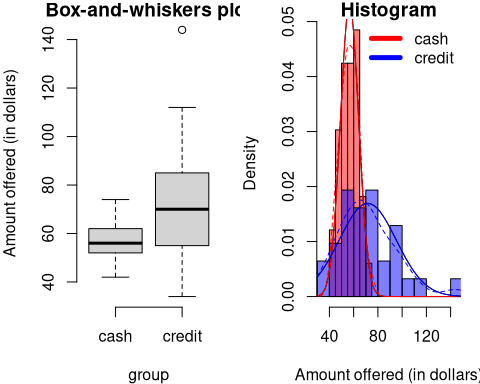
\includegraphics[width=0.7\linewidth]{Statistical-modelling_files/figure-latex/plottickets-1} \end{center}

\begin{Shaded}
\begin{Highlighting}[]
\CommentTok{# Quantile-quantile plots}
\CommentTok{# install `car` package (only once)}
\CommentTok{# uncomment following line to install}
\CommentTok{# install.packages("car")}
\CommentTok{# default function is `qqnorm}
\NormalTok{car}\OperatorTok{::}\KeywordTok{qqPlot}\NormalTok{(offer[group }\OperatorTok{==}\StringTok{ "cash"}\NormalTok{],}
            \DataTypeTok{ylab =} \StringTok{"observed quantiles (cash)"}\NormalTok{)}
\end{Highlighting}
\end{Shaded}

\begin{verbatim}
## [1] 32  8
\end{verbatim}

\begin{Shaded}
\begin{Highlighting}[]
\NormalTok{car}\OperatorTok{::}\KeywordTok{qqPlot}\NormalTok{(offer[group }\OperatorTok{==}\StringTok{ "credit"}\NormalTok{],}
            \DataTypeTok{ylab =} \StringTok{"observed quantiles (credit)"}\NormalTok{)}
\end{Highlighting}
\end{Shaded}

\begin{center}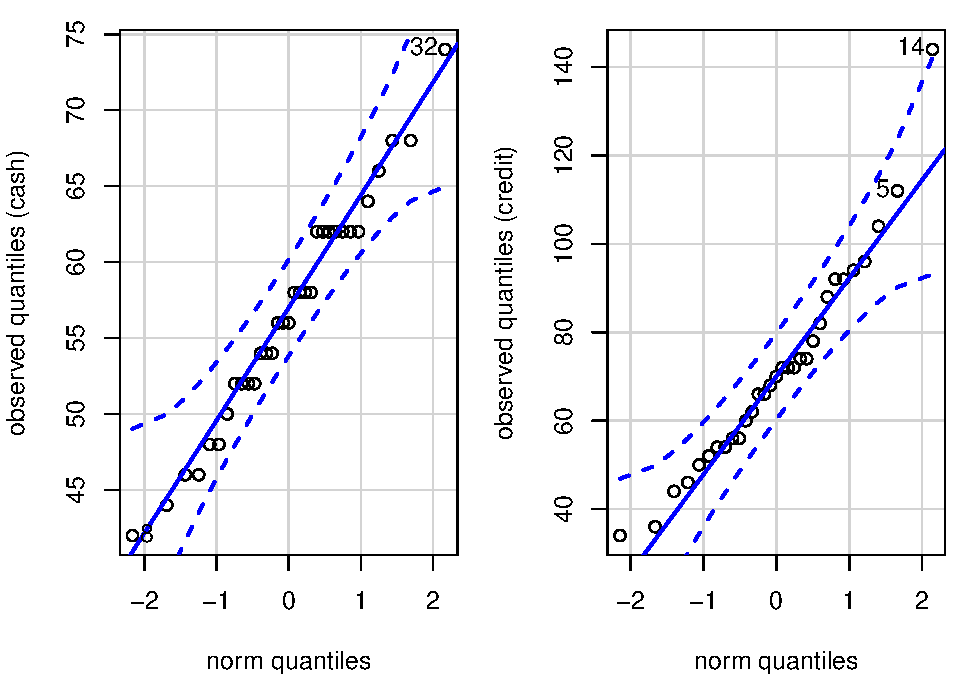
\includegraphics[width=0.7\linewidth]{Statistical-modelling_files/figure-latex/plottickets-2} \end{center}

\begin{verbatim}
## [1] 14  5
\end{verbatim}

\begin{Shaded}
\begin{Highlighting}[]
\CommentTok{# alternatively}
\CommentTok{# qqnorm(offer[group=="cash"], main = "cash")}
\CommentTok{# qqline(offer[group=="cash"])}
\CommentTok{# Detach dataset (don't forget)}
\KeywordTok{detach}\NormalTok{(tickets)}
\end{Highlighting}
\end{Shaded}

\hypertarget{wilcoxon-rank-sum-test}{%
\section{Wilcoxon rank sum test}\label{wilcoxon-rank-sum-test}}

If the data are not normal, either because the distribution is skewed or heavy-tailed, or because the sample sizes are small enough that the asymptotic distribution of the Welch test or the two-sample \(t\)-test is unreliable, we may resort to non-parametric procedures. The Wilcoxon rank-sum test is a test for a shift in distribution; the drawback is that it requires the distribution of the samples to be the same, up to a change in location. If the mean is finite, then this amounts to a change in mean under the assumption that \(F_1(x-\Delta)=F_0(x)\) for any \(x\) for \(F_0, F_1\) the distribution function in group 0 and 1, respectively.

The syntax for the test is analogous to that of the other using the formula \texttt{y\ \textasciitilde{}\ x}, namely \texttt{wilcox.test(offer\ \textasciitilde{}\ groupe,\ data\ =\ tickets)}. You can also specify the values for the two samples with the arguments \texttt{x} and \texttt{y}.
The Wilcoxon rank sum test works with ranks, which is the relative position of the observations in the pooled sample. Intuitively, if there is no difference and both samples come from the same distribution \(F_0(x)\), the sum of the ranks in either group (relative to the number of observations in that group) should not be systematically too large or too small. Because ranks are bounded by \(n\), the test statistic is less sensitive to outliers or extremes, even if its power is not as great in small samples, the loss of power is often not meaningful and the robustness is appealing, which is why Wilcoxon rank sum test is widely used in practice. Since ranks are discrete, the distribution of the sum is tractable and we can use combinatorics to list all possibilities. For example, with eight observations split in two subgroups of equal size, the null distribution is

10

11

12

13

14

15

16

17

18

19

20

21

22

23

24

25

26

Probability (\%)

1.4

1.4

2.9

4.3

7.1

7.1

10

10

11

10

10

7.1

7.1

4.3

2.9

1.4

1.4

Note that the value returned by \textbf{R} for the Wilcoxon rank sum test is not the same as the formula covered in class; it subtracts the minimum possible rank sum, here \(m(m+1)/2\) for a first sample of size \(m\) so that the statistic is bounded below by zero, regardless of the sample size. As this is a shift by a deterministic constant, it has no impact on the asymptotic distribution.

In practice, there will often be ties (when two values are identical) and this means that the ranks are not uniquely defined (we could assign ranks at random for ties, or take the average, etc.); \textbf{R} will print a warning message to notify the user of the presence of ties. Formulae are adapted to deal with ties, but the software computes these automatically for us. While you will see multiple online references to the function \texttt{wilcox.test}, it does not return the correct \(p\)-value, point estimate or confidence interval as soon as there are ties --- it is unfortunately is not doing the right thing. Outside of small samples, tabulating the null distribution is prohibitive if there are more than 50 observations in total, since the total number of possibilities explodes. In class, we saw that a normal approximation for the null distribution, i.e., the distribution of the rank sum test under the assumption that the two samples, of size \(n_1\) and \(n-n_1=n_2\), respectively, both have distribution function \(F\). The distribution can easily be approximated by simulation, by sampling uniformly integer values from 1 to \(n\) and summing the first \(n_1\). We can repeat this a large number of times and get a good approximation. If there are ties, we proceed accordingly by resampling \(n_1\) of the \(n\) ranks, without replacement. The normal approximation, whose formula was given in the slides, matches quite closely the empirical distribution of the simulated values; this is a consequence of the central limit theorem. Because of the normal approximation, we can do two-sided tests exactly as before by defining exteme values as deviation from the mean either side.

We illustrate this concept with the \texttt{tickets} data; bear in mind that the test is not valid here, because the data clearly do not come from the same distribution up to a shift (in particular, the variance are clearly not the same). We would normally need to test formally for equality of distribution up to a location shift, but this requires yet another test; most of the time, we will assess this hypothesis graphically.

\begin{Shaded}
\begin{Highlighting}[]
\NormalTok{n <-}\StringTok{ }\KeywordTok{nrow}\NormalTok{(tickets)}
\CommentTok{# correct p-value, wrong confint and pe}
\NormalTok{exactRankTests}\OperatorTok{::}\KeywordTok{wilcox.exact}\NormalTok{(offer }\OperatorTok{~}\StringTok{ }\NormalTok{group, }\DataTypeTok{data =}\NormalTok{ tickets, }\DataTypeTok{conf.int =} \OtherTok{TRUE}\NormalTok{)}
\end{Highlighting}
\end{Shaded}

\begin{verbatim}
## 
##  Exact Wilcoxon rank sum test
## 
## data:  offer by group
## W = 288, p-value = 0.002
## alternative hypothesis: true mu is not equal to 0
## 95 percent confidence interval:
##  -22  -4
## sample estimates:
## difference in location 
##                    -13
\end{verbatim}

\begin{Shaded}
\begin{Highlighting}[]
\CommentTok{# wrong p-value b/c of ties, correct confint and pe}
\KeywordTok{wilcox.test}\NormalTok{(offer }\OperatorTok{~}\StringTok{ }\NormalTok{group, }\DataTypeTok{data =}\NormalTok{ tickets, }\DataTypeTok{conf.int =} \OtherTok{TRUE}\NormalTok{)}
\end{Highlighting}
\end{Shaded}

\begin{verbatim}
## 
##  Wilcoxon rank sum test with continuity correction
## 
## data:  offer by group
## W = 288, p-value = 0.003
## alternative hypothesis: true location shift is not equal to 0
## 95 percent confidence interval:
##  -20  -4
## sample estimates:
## difference in location 
##                    -12
\end{verbatim}

\begin{Shaded}
\begin{Highlighting}[]
\CommentTok{# Test statistic is sum of ranks}
\NormalTok{Wteststat <-}\StringTok{ }\KeywordTok{sum}\NormalTok{(}\KeywordTok{rank}\NormalTok{(tickets}\OperatorTok{$}\NormalTok{offer, }
                      \DataTypeTok{ties.method =} \StringTok{"average"}\NormalTok{)[tickets}\OperatorTok{$}\NormalTok{group }\OperatorTok{==}\StringTok{ "cash"}\NormalTok{])}
         
\CommentTok{# Compute the p-value through simulation}
\NormalTok{prank <-}\StringTok{ }\KeywordTok{rank}\NormalTok{(tickets}\OperatorTok{$}\NormalTok{offer, }
             \DataTypeTok{ties.method =} \StringTok{"average"}\NormalTok{)}
\NormalTok{nrep <-}\StringTok{ }\FloatTok{1e6}\NormalTok{L}
\NormalTok{W <-}\StringTok{ }\KeywordTok{rep}\NormalTok{(}\DecValTok{0}\NormalTok{, nrep)}
\ControlFlowTok{for}\NormalTok{(i }\ControlFlowTok{in} \DecValTok{1}\OperatorTok{:}\NormalTok{nrep)\{}
   \CommentTok{#resample the ranks}
\NormalTok{   x <-}\StringTok{ }\KeywordTok{sample}\NormalTok{(prank, }\DataTypeTok{size =} \DecValTok{33}\NormalTok{, }\DataTypeTok{replace =} \OtherTok{FALSE}\NormalTok{)}
\NormalTok{   W[i] <-}\StringTok{ }\KeywordTok{sum}\NormalTok{(x)}
\NormalTok{\}}
\NormalTok{n1 <-}\StringTok{ }\DecValTok{33}\NormalTok{; }
\NormalTok{n2 <-}\StringTok{ }\DecValTok{31}

\KeywordTok{hist}\NormalTok{(W, }\DataTypeTok{freq =} \OtherTok{FALSE}\NormalTok{, }
     \DataTypeTok{ylab =} \StringTok{"density"}\NormalTok{, }
     \DataTypeTok{xlab =} \StringTok{"simulated $W$"}\NormalTok{, }
     \DataTypeTok{main =} \StringTok{""}\NormalTok{) }\CommentTok{#remove title}
\KeywordTok{abline}\NormalTok{(}\DataTypeTok{v =}\NormalTok{ Wteststat, }\DataTypeTok{col =} \StringTok{"red"}\NormalTok{)}\CommentTok{# add line for test stat}

\CommentTok{# Warning: this normal approximation is for}
\CommentTok{# data w/o ties, i.e., the formula presented}
\CommentTok{# in the course slides }
\NormalTok{mues <-}\StringTok{ }\NormalTok{n1}\OperatorTok{*}\NormalTok{(n1}\OperatorTok{+}\NormalTok{n2}\OperatorTok{+}\DecValTok{1}\NormalTok{)}\OperatorTok{/}\DecValTok{2} \CommentTok{#mean of normal approx}
\NormalTok{sdes <-}\StringTok{ }\KeywordTok{sqrt}\NormalTok{(n1}\OperatorTok{*}\NormalTok{n2}\OperatorTok{*}\NormalTok{(n1}\OperatorTok{+}\NormalTok{n2}\OperatorTok{+}\DecValTok{1}\NormalTok{)}\OperatorTok{/}\DecValTok{12}\NormalTok{) }\CommentTok{#var of normal approx}
\CommentTok{#superimpose normal approx to empirical distribution}
\KeywordTok{lines}\NormalTok{(}\KeywordTok{seq}\NormalTok{(}\DecValTok{700}\NormalTok{, }\DecValTok{1600}\NormalTok{, }\DataTypeTok{length =}\NormalTok{ 1000L),}
\KeywordTok{dnorm}\NormalTok{(x <-}\StringTok{ }\KeywordTok{seq}\NormalTok{(}\DecValTok{700}\NormalTok{, }\DecValTok{1600}\NormalTok{, }\DataTypeTok{length =}\NormalTok{ 1000L),}
      \DataTypeTok{mean =}\NormalTok{ mues, }\DataTypeTok{sd =}\NormalTok{ sdes), }\DataTypeTok{lwd =} \DecValTok{2}\NormalTok{, }\DataTypeTok{col =} \DecValTok{4}\NormalTok{)}
\end{Highlighting}
\end{Shaded}

\begin{center}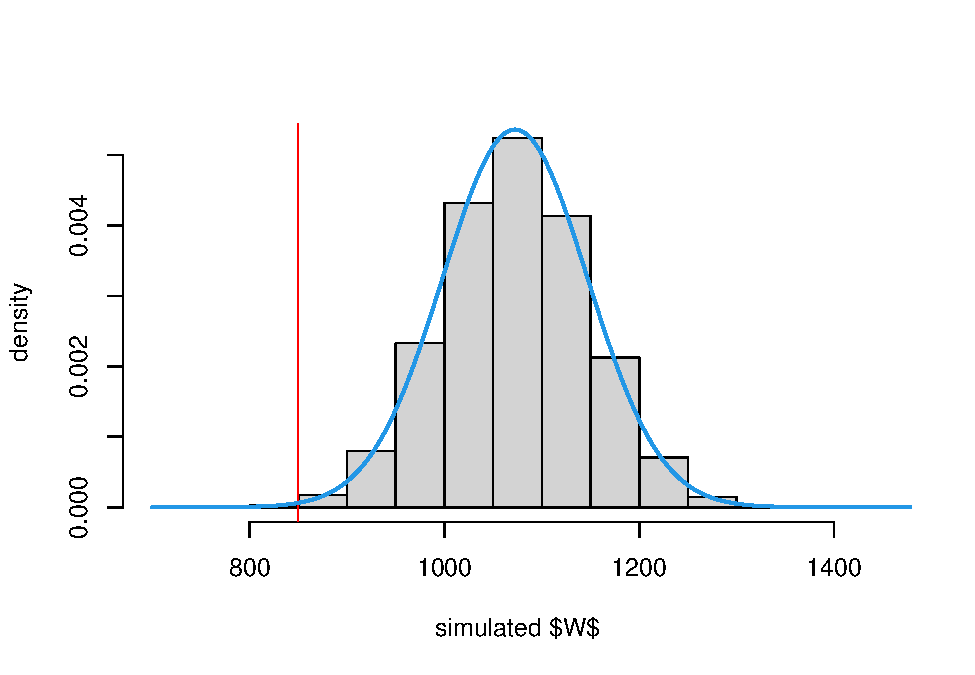
\includegraphics[width=0.7\linewidth]{Statistical-modelling_files/figure-latex/wilcoxsimu-1} \end{center}

\begin{Shaded}
\begin{Highlighting}[]
\CommentTok{# Simulated one-sided p-value}
\CommentTok{# by defn, proportion of samples as extreme (i.e. smaller)}
\KeywordTok{mean}\NormalTok{(W }\OperatorTok{<}\StringTok{ }\NormalTok{Wteststat)}
\end{Highlighting}
\end{Shaded}

\begin{verbatim}
## [1] 0.0011
\end{verbatim}

\begin{Shaded}
\begin{Highlighting}[]
\CommentTok{#p-value from normal approx}
\KeywordTok{pnorm}\NormalTok{(}\DataTypeTok{q =}\NormalTok{ Wteststat, }\DataTypeTok{mean =}\NormalTok{ mues, }\DataTypeTok{sd =}\NormalTok{ sdes)}
\end{Highlighting}
\end{Shaded}

\begin{verbatim}
## [1] 0.0014
\end{verbatim}

\begin{Shaded}
\begin{Highlighting}[]
\CommentTok{# One sided confidence interval based on normal approx.}
\NormalTok{mues}\OperatorTok{-}\KeywordTok{qnorm}\NormalTok{(}\FloatTok{0.95}\NormalTok{)}\OperatorTok{*}\NormalTok{sdes}
\end{Highlighting}
\end{Shaded}

\begin{verbatim}
## [1] 950
\end{verbatim}

The value returned for the \(p\)-value by \texttt{wilcox.exact} would be roughly twice the one-sided \(p\)-value, in this case. The normal approximation is also convenient for obtaining confidence intervals, here {[}950.06, \(\infty\)).

The \texttt{wilcox.test} function returns the so-called Hodges--Lehmann estimator (i.e., the median of all the pairs \(Y^{(1)}_i-Y^{(2)}_j\) (\(i=1, \ldots, n_1\); \(j=1, \ldots, n_2\)). These point estimators, the associated confidence intervals and the exact coverage of the intervals (with additionally the subtleties surrounging from ties and zeros) are beyond the scope of the course, but \href{http://www.stat.umn.edu/geyer/5601/examp/ranksum.html}{Charles Geyer's course notes give additional information}. The following function is adapted from his code and is distributed under \href{https://creativecommons.org/licenses/by-sa/3.0/}{CC BY-SA 3.0} licence. It can be used to compute the Hodges--Lehmann estimator with the associated confidence interval, while also returning the coverage (not exactly 95\% because of the discreteness of the data).

\begin{Shaded}
\begin{Highlighting}[]
\KeywordTok{source}\NormalTok{(}\StringTok{"https://lbelzile.bitbucket.io/MATH60619A/hl_wilcox.R"}\NormalTok{)}
\NormalTok{hl <-}\StringTok{ }\KeywordTok{hl.wilcox}\NormalTok{(tickets}\OperatorTok{$}\NormalTok{offer[tickets}\OperatorTok{$}\NormalTok{group }\OperatorTok{==}\StringTok{ "credit"}\NormalTok{], }
\NormalTok{          tickets}\OperatorTok{$}\NormalTok{offer[tickets}\OperatorTok{$}\NormalTok{group }\OperatorTok{==}\StringTok{ "cash"}\NormalTok{])}
\end{Highlighting}
\end{Shaded}

\begin{verbatim}
## Wilcoxon rank sum test 
## Hodges-Lehmann estimator:  -12 
## confidence interval:  -20 -4 
## achieved confidence level: 0.95
\end{verbatim}

Another potential nonparametric test is the Fligner--Policello test. Unlike Wilcoxon rank sum, it does not assume that the two distributions are equal under the null hypothesis, but require them to be symmetrical around their median (so the variance in each group could be different). \href{http://support.sas.com/documentation/cdl/en/statug/67523/HTML/default/viewer.htm\#statug_npar1way_details20.htm}{\textbf{SAS} implements the test and uses the asymptotic normal approximation for \emph{p} values and such like}.

In \textbf{R}, the \texttt{NSM3} package provides an implementation of the Fligner--Policello test.

\begin{Shaded}
\begin{Highlighting}[]
\NormalTok{fptest <-}\StringTok{ }\NormalTok{NSM3}\OperatorTok{::}\KeywordTok{pFligPoli}\NormalTok{(tickets}\OperatorTok{$}\NormalTok{offer[tickets}\OperatorTok{$}\NormalTok{group }\OperatorTok{==}\StringTok{ "credit"}\NormalTok{], }
\NormalTok{          tickets}\OperatorTok{$}\NormalTok{offer[tickets}\OperatorTok{$}\NormalTok{group }\OperatorTok{==}\StringTok{ "cash"}\NormalTok{])}
\DecValTok{1}\OperatorTok{-}\NormalTok{fptest}\OperatorTok{$}\NormalTok{p.val}
\end{Highlighting}
\end{Shaded}

\begin{verbatim}
## [1] 0.0028
\end{verbatim}

The estimated \(p\)-value for the one-sided test is \(0.0017\).

\hypertarget{linear-regression}{%
\chapter{Linear regression}\label{linear-regression}}

In class, we conducted an analysis of the linear relation between buying intention for customers (\texttt{intention}) and the number of seconds the subject fixated a candy advertisement (\texttt{fixation}) using a simple linear regression. The following noes will show you how to do this using \textbf{R}. Normally, strings are cast to factor (unless you specify \texttt{stringsAsFactors\ =\ FALSE}), but the danger here is that some variables are encoded using integers (sex, revenue, level of education, marital status). It is okay if we keep binary variables, i.e., those encoded as 0-1, as is, but it is often better to cast them to factor to get more meaningful labels given the lack of obvious ordering. Note that response variable intention is bounded between \([2, 14]\) by construction, being the sum of two Likert scales ranging from 1 to 7. The normal approximation with a sample size this large probably means this won't impact the inference, but we must be careful with predictions (by truncating them lie within the range of possible values).

\begin{Shaded}
\begin{Highlighting}[]
\NormalTok{url <-}\StringTok{ "https://lbelzile.bitbucket.io/MATH60619A/intention.txt"}
\NormalTok{intention <-}\StringTok{ }\KeywordTok{read.table}\NormalTok{(url, }\DataTypeTok{header =} \OtherTok{TRUE}\NormalTok{)}
\CommentTok{# number of observations (rows) and variables (cols)}
\KeywordTok{dim}\NormalTok{(intention) }
\end{Highlighting}
\end{Shaded}

\begin{verbatim}
## [1] 120  10
\end{verbatim}

\begin{Shaded}
\begin{Highlighting}[]
\KeywordTok{summary}\NormalTok{(intention)}
\end{Highlighting}
\end{Shaded}

\begin{verbatim}
##     fixation      emotion          sex            age        revenue    
##  Min.   :0.0   Min.   :0.05   Min.   :0.00   Min.   :19   Min.   :1.00  
##  1st Qu.:0.8   1st Qu.:0.72   1st Qu.:0.00   1st Qu.:27   1st Qu.:1.00  
##  Median :1.3   Median :0.93   Median :1.00   Median :30   Median :2.00  
##  Mean   :1.6   Mean   :1.04   Mean   :0.52   Mean   :30   Mean   :2.07  
##  3rd Qu.:2.1   3rd Qu.:1.38   3rd Qu.:1.00   3rd Qu.:33   3rd Qu.:3.00  
##  Max.   :5.8   Max.   :2.80   Max.   :1.00   Max.   :45   Max.   :3.00  
##       educ         marital       intention         buy           nitem     
##  Min.   :1.00   Min.   :0.00   Min.   : 2.0   Min.   :0.00   Min.   : 0.0  
##  1st Qu.:1.75   1st Qu.:0.00   1st Qu.: 6.0   1st Qu.:0.00   1st Qu.: 0.0  
##  Median :2.00   Median :1.00   Median : 8.0   Median :0.00   Median : 0.0  
##  Mean   :2.04   Mean   :0.54   Mean   : 8.3   Mean   :0.45   Mean   : 1.7  
##  3rd Qu.:3.00   3rd Qu.:1.00   3rd Qu.:11.0   3rd Qu.:1.00   3rd Qu.: 2.0  
##  Max.   :3.00   Max.   :1.00   Max.   :14.0   Max.   :1.00   Max.   :10.0
\end{verbatim}

\begin{Shaded}
\begin{Highlighting}[]
\CommentTok{#variable names}
\KeywordTok{colnames}\NormalTok{(intention)}
\end{Highlighting}
\end{Shaded}

\begin{verbatim}
##  [1] "fixation"  "emotion"   "sex"       "age"       "revenue"   "educ"     
##  [7] "marital"   "intention" "buy"       "nitem"
\end{verbatim}

\begin{Shaded}
\begin{Highlighting}[]
\CommentTok{# cast categorical and ordinal variables to factors}
\NormalTok{intention}\OperatorTok{$}\NormalTok{revenue <-}\StringTok{ }\KeywordTok{factor}\NormalTok{(intention}\OperatorTok{$}\NormalTok{revenue, }
                            \DataTypeTok{labels =} \KeywordTok{c}\NormalTok{(}\StringTok{'low'}\NormalTok{,}\StringTok{'medium'}\NormalTok{,}\StringTok{'high'}\NormalTok{),}
                             \DataTypeTok{ordered =} \OtherTok{TRUE}\NormalTok{)}
\NormalTok{intention}\OperatorTok{$}\NormalTok{educ <-}\StringTok{ }\KeywordTok{factor}\NormalTok{(intention}\OperatorTok{$}\NormalTok{educ, }
                            \DataTypeTok{labels =} \KeywordTok{c}\NormalTok{(}\StringTok{' <high school'}\NormalTok{,}\StringTok{'high school'}\NormalTok{,}\StringTok{'university'}\NormalTok{))}
\NormalTok{intention}\OperatorTok{$}\NormalTok{marital <-}\StringTok{ }\KeywordTok{factor}\NormalTok{(intention}\OperatorTok{$}\NormalTok{marital,}
                            \DataTypeTok{labels =} \KeywordTok{c}\NormalTok{(}\StringTok{"single"}\NormalTok{,}\StringTok{"relationship"}\NormalTok{))}
\NormalTok{intention}\OperatorTok{$}\NormalTok{sex <-}\StringTok{ }\KeywordTok{factor}\NormalTok{(intention}\OperatorTok{$}\NormalTok{sex, }
                           \DataTypeTok{labels =} \KeywordTok{c}\NormalTok{(}\StringTok{"man"}\NormalTok{,}\StringTok{"woman"}\NormalTok{))}
\end{Highlighting}
\end{Shaded}

By default, the baseline level for a factor is based on the alphabetical order, while \textbf{SAS} uses the first value it encounters (?). Once the variables are cast to factor, \texttt{summary} will print the counts for each respective categories; these could be likewise be obtained using \texttt{table}.

Before fitting a simple linear regression model, we should assess whether there is a linear relationship between the response and the explanatory (or not); a scatterplot can help to assess this. We superimpose the least square fit to the plot. In both cases, there is some positive correlation between intention and the explanatories, but this correlation is weak.

\begin{Shaded}
\begin{Highlighting}[]
\KeywordTok{par}\NormalTok{(}\DataTypeTok{mfrow=}\KeywordTok{c}\NormalTok{(}\DecValTok{1}\NormalTok{,}\DecValTok{2}\NormalTok{), }\DataTypeTok{pch =} \DecValTok{20}\NormalTok{, }\DataTypeTok{bty =} \StringTok{'l'}\NormalTok{)}
\KeywordTok{plot}\NormalTok{(intention }\OperatorTok{~}\StringTok{ }\NormalTok{fixation, }\DataTypeTok{data =}\NormalTok{ intention)}
\KeywordTok{abline}\NormalTok{(}\KeywordTok{lm}\NormalTok{(intention }\OperatorTok{~}\StringTok{ }\NormalTok{fixation, }\DataTypeTok{data =}\NormalTok{ intention))}
\KeywordTok{plot}\NormalTok{(intention }\OperatorTok{~}\StringTok{ }\NormalTok{emotion, }\DataTypeTok{data =}\NormalTok{ intention)}
\KeywordTok{abline}\NormalTok{(}\KeywordTok{lm}\NormalTok{(intention }\OperatorTok{~}\StringTok{ }\NormalTok{emotion, }\DataTypeTok{data =}\NormalTok{ intention))}
\end{Highlighting}
\end{Shaded}

\begin{center}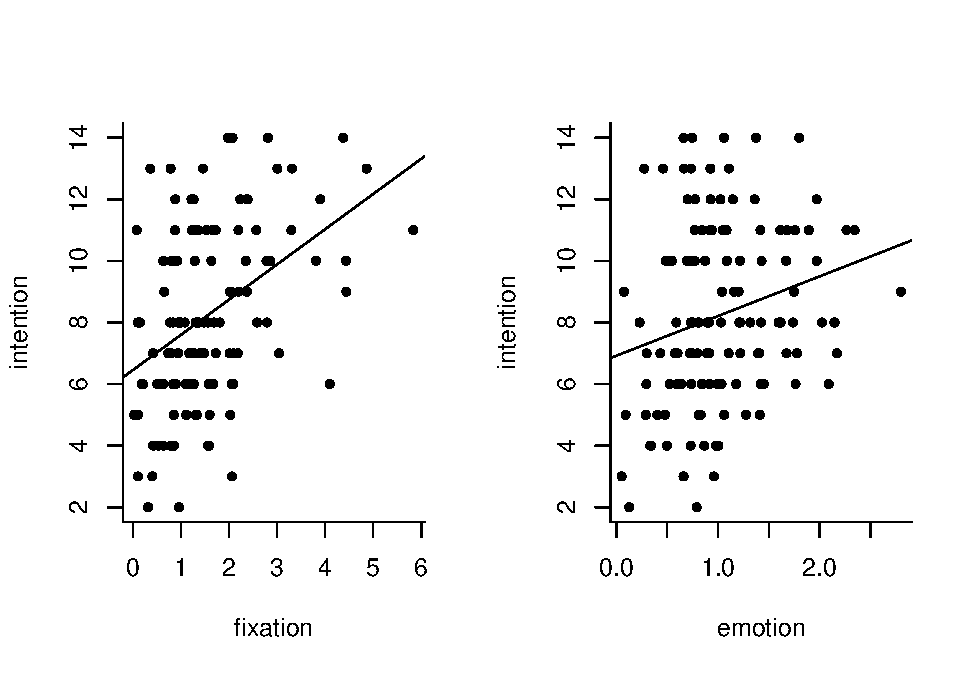
\includegraphics[width=0.7\linewidth]{Statistical-modelling_files/figure-latex/slrscatterplots-1} \end{center}

We can compute the correlation coefficient using \texttt{cor}; we get 0.43 for \texttt{intention} and \texttt{fixation} and 0.23 for \texttt{intention} and \texttt{emotion}. If we specify a matrix with more than two columns or a data frame (with numeric values), we get a correlation matrix with ones on the diagonal. For factor variables, we would need to map these back to binary, but we saw that the \(R^2\) value is equal to the squared correlation coefficient, so we can extract this from the output of the linear model fit.

\hypertarget{the-lm-function}{%
\section{\texorpdfstring{The \texttt{lm} function}{The lm function}}\label{the-lm-function}}

The function \texttt{lm} is the workshorse for fitting linear models. It takes as input a formula: suppose you have a data frame containing columns \texttt{x} (a regressor) and \texttt{y} (the regressand); you can then call \texttt{lm(y\ \textasciitilde{}\ x)} to fit the linear model \(y = \beta_0 + \beta_1 x + \varepsilon\). The explanatory variable \texttt{y} is on the left hand side,
while the right hand side should contain the predictors, separated by a \texttt{+} sign if there are more than one.
If you provide the data frame name using \texttt{data}, then the shorthand \texttt{y\ \textasciitilde{}\ .} fits all the columns of the data frame (but \texttt{y}) as regressors.

To fit higher order polynomials or transformations, use the \texttt{I} function to tell \textbf{R} to interpret the input ``as is''.
Thus, \texttt{lm(y\textasciitilde{}x+I(x\^{}2))}, would fit a linear model with design matrix \((\boldsymbol{1}_n, \mathbf{x}^\top, \mathbf{x}^2)^\top\). A constant is automatically included in the regression, but can be removed by writing \texttt{-1} or \texttt{+0} on the right hand side of the formula.

The \texttt{lm} function output will display ordinary least squares estimates along with standard errors, \(t\) values for the Wald test of the hypothesis \(\mathrm{H}_0: \beta_i=0\) and the associated \(P\)-values. Other statistics and information about the sample size, the degrees of freedom, etc., are given at the bottom of the table.

Many methods allow you to extract specific objects. For example, the functions \texttt{coef}, \texttt{resid}, \texttt{fitted}, \texttt{model.matrix} will return \(\widehat{\boldsymbol{\beta}}\), \(\boldsymbol{e}\), \(\widehat{\boldsymbol{y}}\) and \(\mathbf{X}\), respectively.

\begin{Shaded}
\begin{Highlighting}[]
\NormalTok{linmod <-}\StringTok{ }\KeywordTok{lm}\NormalTok{(intention }\OperatorTok{~}\StringTok{ }\NormalTok{fixation, }\DataTypeTok{data =}\NormalTok{ intention)}
\KeywordTok{summary}\NormalTok{(linmod)}
\end{Highlighting}
\end{Shaded}

\begin{verbatim}
## 
## Call:
## lm(formula = intention ~ fixation, data = intention)
## 
## Residuals:
##    Min     1Q Median     3Q    Max 
## -5.813 -1.828 -0.207  2.176  6.130 
## 
## Coefficients:
##             Estimate Std. Error t value Pr(>|t|)    
## (Intercept)    6.453      0.428   15.06  < 2e-16 ***
## fixation       1.144      0.224    5.12  1.2e-06 ***
## ---
## Signif. codes:  0 '***' 0.001 '**' 0.01 '*' 0.05 '.' 0.1 ' ' 1
## 
## Residual standard error: 2.7 on 118 degrees of freedom
## Multiple R-squared:  0.182,  Adjusted R-squared:  0.175 
## F-statistic: 26.2 on 1 and 118 DF,  p-value: 1.21e-06
\end{verbatim}

\begin{Shaded}
\begin{Highlighting}[]
\KeywordTok{confint}\NormalTok{(linmod) }\CommentTok{#confidence intervals for model parameters}
\end{Highlighting}
\end{Shaded}

\begin{verbatim}
##             2.5 % 97.5 %
## (Intercept)   5.6    7.3
## fixation      0.7    1.6
\end{verbatim}

\begin{Shaded}
\begin{Highlighting}[]
\NormalTok{yhat <-}\StringTok{ }\KeywordTok{fitted}\NormalTok{(linmod) }\CommentTok{#fitted values yhat}
\NormalTok{e <-}\StringTok{ }\KeywordTok{resid}\NormalTok{(linmod) }\CommentTok{#ordinary residuals}
\NormalTok{jsr <-}\StringTok{ }\KeywordTok{rstudent}\NormalTok{(linmod) }\CommentTok{#jackknife studentized resid.}
\end{Highlighting}
\end{Shaded}

The estimated intercept \(\widehat{\beta}_0\) is 6.92 and the estimated slope \(\widehat{\beta}_1\) is 1.29 The table gives the \(p\)-values for the null hypotheses \(\beta_0=0\) and \(\beta_1=0\), which are negligible. The estimated variance \(\widehat{\sigma}^2\), given by the \texttt{Residual\ standard\ error} is 2.86.

To obtain predicted values for combination of explanatories not present in the dataset, we need to first create a new data frame, with the same column names as those of the explanatory. In this case, the only \(\mathrm{X}\) variable is \texttt{fixation}. We can get confidence intervals for the mean value with \texttt{interval\ =\ "conf"} or prediction intervals for the new observations with \texttt{interval\ =\ "pred"}.

\begin{Shaded}
\begin{Highlighting}[]
\NormalTok{newdata <-}\StringTok{ }\KeywordTok{data.frame}\NormalTok{(}\DataTypeTok{fixation =} \KeywordTok{seq}\NormalTok{(}\DecValTok{0}\NormalTok{, }\FloatTok{6.5}\NormalTok{, }\DataTypeTok{length.out =}\NormalTok{ 100L))}
\CommentTok{# Predictions with confidence interval for E(Y)}
\NormalTok{fitted_vals <-}\StringTok{ }\KeywordTok{predict}\NormalTok{(}\DataTypeTok{object =}\NormalTok{ linmod, }
         \DataTypeTok{newdata =}\NormalTok{ newdata, }
         \DataTypeTok{interval =} \StringTok{"conf"}\NormalTok{)}
\CommentTok{#Same, but with prediction intervals for Y_new}
\NormalTok{predict_vals <-}\StringTok{ }\KeywordTok{predict}\NormalTok{(}\DataTypeTok{object =}\NormalTok{ linmod, }
         \DataTypeTok{newdata =}\NormalTok{ newdata, }
         \DataTypeTok{interval =} \StringTok{"pred"}\NormalTok{)}
\KeywordTok{plot}\NormalTok{(intention }\OperatorTok{~}\StringTok{ }\NormalTok{fixation, }\DataTypeTok{data =}\NormalTok{ intention)}
\KeywordTok{matplot}\NormalTok{(}\DataTypeTok{x =}\NormalTok{ newdata}\OperatorTok{$}\NormalTok{fixation,}
        \DataTypeTok{y =}\NormalTok{ fitted_vals, }
        \DataTypeTok{col =} \StringTok{"blue"}\NormalTok{, }
        \DataTypeTok{add =} \OtherTok{TRUE}\NormalTok{,}
        \DataTypeTok{type =} \StringTok{"l"}\NormalTok{)}
\KeywordTok{matplot}\NormalTok{(}\DataTypeTok{x =}\NormalTok{ newdata}\OperatorTok{$}\NormalTok{fixation,}
        \DataTypeTok{y =}\NormalTok{ predict_vals, }
        \DataTypeTok{lty =} \DecValTok{2}\NormalTok{, }\CommentTok{#dashed lines, }
        \DataTypeTok{col =} \StringTok{"blue"}\NormalTok{, }
        \DataTypeTok{add =} \OtherTok{TRUE}\NormalTok{,}
        \DataTypeTok{type =} \StringTok{"l"}\NormalTok{)}
\end{Highlighting}
\end{Shaded}

\begin{center}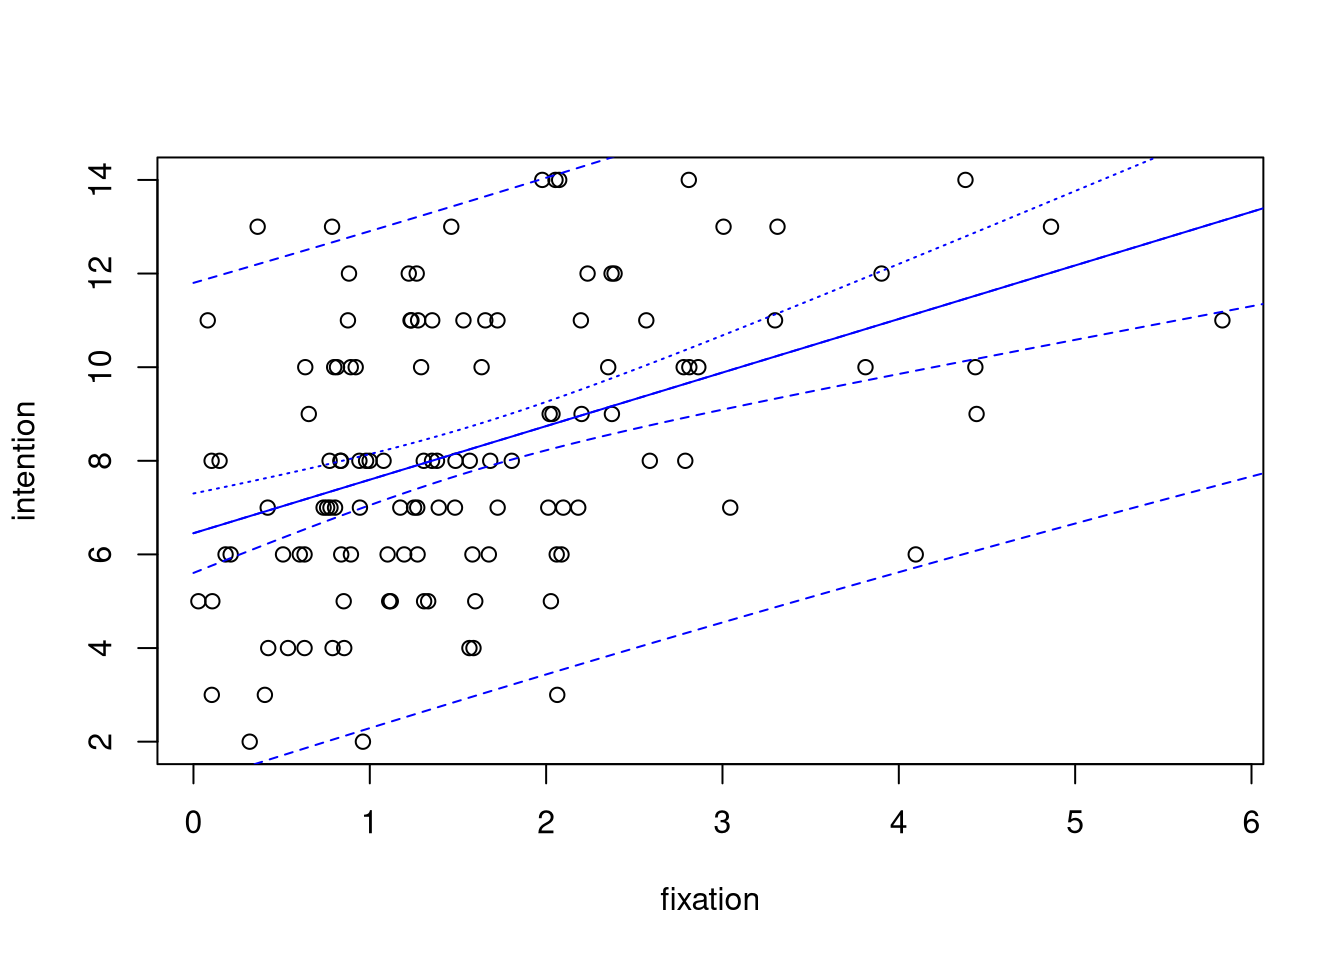
\includegraphics[width=0.7\linewidth]{Statistical-modelling_files/figure-latex/plotfitted-1} \end{center}

The confidence interval for the mean value \(\mathsf{E}({\widehat{Y}_i})\) is larger for values of \(\mathrm{X}\) that are far from \(\overline{\mathrm{X}}\); since there are less neighboring points, the model is extrapolating at this point and this translates in higher uncertainty, roughly speaking. The prediction intervals are much wider and account for the additional variability of \(\varepsilon_{\text{new}}\); the intervals are pointwise, so for any given \(\mathrm{X}\), we would assume that 95\% of the intervals in repeated samples would capture \(Y_{\text{new}}\).

\hypertarget{graphical-diagnostics-and-analysis-of-residuals}{%
\subsection{Graphical diagnostics and analysis of residuals}\label{graphical-diagnostics-and-analysis-of-residuals}}

The hypothesis underlying the classical linear model are

\begin{enumerate}
\def\labelenumi{\arabic{enumi}.}
\tightlist
\item
  independence
\item
  linearity (correct specification of the mean response)
\item
  homoscedasticity
\item
  normality
\end{enumerate}

Underlying the linear model
\begin{align*}
Y_i = \beta_0 + \sum_{j=1}^p \mathrm{X}_{ij} + \varepsilon_i.
\end{align*}
is the hypothesis that the errors \(\{\varepsilon_i\}_{i=1}^n\) are independent and identically distributed \(\mathcal{N}(0, \sigma^2)\) variables. We get to observe \(y_i (i=1,\ldots,n)\), but \(\beta_0, \beta_1, \ldots \beta_p, \sigma^2, \varepsilon_i (i=1,\ldots,n)\) are all unknown. The best we can hope for is
least square estimates for \(\beta\)'s, say \(\widehat{\beta}_0, \ldots, \widehat{\beta}_p\).
The fitted values are \(\widehat{y}_i=\widehat{\beta}_0 + \sum_{j=1}^p \widehat{\beta}_j \mathrm{X}_{i,j}\) from which we will deduce the \textbf{ordinary residuals} \(e_i = Y_i - \widehat{Y}_i\).

Unfortunately, it turns out that \(e_i\)'s are not independent; worst, they each have a different variance. However, the ordinary residuals and the fitted values are orthogonal, i.e.~their linear correlation is zero. This is also true of \(\mathbf{X}_j\) and \(\boldsymbol{e}\), and \(\overline{e} = 0\) by construction. Thus, if we fit a linear model with mean structure \(\mathsf{E}(e_i) = \beta_0 + \beta_1\mathrm{X}_{ij}\) or \(\mathsf{E}(e_i) = \beta_0 + \beta_1 \widehat{y}_i\), the estimates for \(\widehat{\beta}_0\) and \(\widehat{\beta}_1\) will be exactly zero in both cases. We can verify this numerically.

\begin{Shaded}
\begin{Highlighting}[]
\CommentTok{#check whether coefs are zero}
\KeywordTok{isTRUE}\NormalTok{(}\KeywordTok{all.equal}\NormalTok{(}\KeywordTok{coef}\NormalTok{(}\KeywordTok{lm}\NormalTok{(e }\OperatorTok{~}\StringTok{ }\NormalTok{yhat)), }\KeywordTok{rep}\NormalTok{(}\DecValTok{0}\NormalTok{, }\DecValTok{2}\NormalTok{), }\DataTypeTok{check.attributes =} \OtherTok{FALSE}\NormalTok{))}
\end{Highlighting}
\end{Shaded}

\begin{verbatim}
## [1] TRUE
\end{verbatim}

\begin{Shaded}
\begin{Highlighting}[]
\CommentTok{#due to machine precision, could be ~1e-17}
\KeywordTok{coef}\NormalTok{(}\KeywordTok{lm}\NormalTok{(e }\OperatorTok{~}\StringTok{ }\NormalTok{fixation, }\DataTypeTok{data =}\NormalTok{ intention))}
\end{Highlighting}
\end{Shaded}

\begin{verbatim}
## (Intercept)    fixation 
##    -6.3e-17     8.0e-18
\end{verbatim}

\begin{Shaded}
\begin{Highlighting}[]
\KeywordTok{mean}\NormalTok{(e)}
\end{Highlighting}
\end{Shaded}

\begin{verbatim}
## [1] -4.4e-17
\end{verbatim}

If we plot \(e_i\) against \(\hat{y}_i\) or \(\mathrm{X}_i\), we would expect to see no pattern. If we omitted important explanatory models for \(Y\), these would not be accounted for in the mean model and their impact would be transferred to the residuals, which would be correlated with the omitted covariate. We can use local smoothing to check for residual nonlinear relationships or changepoints between \(e_i\) and \(\hat{y}_i\) or \(e_i\) and \(\mathrm{X}_{i}\) by using a local smoother (LOESS) that should capture these local effects, if present. Bear in mind that the model is not reliable.

\begin{Shaded}
\begin{Highlighting}[]
\KeywordTok{par}\NormalTok{(}\DataTypeTok{mfrow =} \KeywordTok{c}\NormalTok{(}\DecValTok{1}\NormalTok{, }\DecValTok{3}\NormalTok{))}
\NormalTok{car}\OperatorTok{::}\KeywordTok{residualPlot}\NormalTok{(linmod)}
\KeywordTok{scatter.smooth}\NormalTok{(e }\OperatorTok{~}\StringTok{ }\NormalTok{intention}\OperatorTok{$}\NormalTok{fixation, }
     \DataTypeTok{xlab =} \StringTok{"fixation (in sec)"}\NormalTok{,}
     \DataTypeTok{ylab =} \StringTok{"ordinary residuals"}\NormalTok{)}
\KeywordTok{scatter.smooth}\NormalTok{(e }\OperatorTok{~}\StringTok{ }\NormalTok{intention}\OperatorTok{$}\NormalTok{emotion, }
     \DataTypeTok{xlab =} \StringTok{"omitted covariate}\CharTok{\textbackslash{}n}\StringTok{`emotion`"}\NormalTok{,}
     \DataTypeTok{ylab =} \StringTok{"ordinary residuals"}\NormalTok{)}
\end{Highlighting}
\end{Shaded}

\begin{center}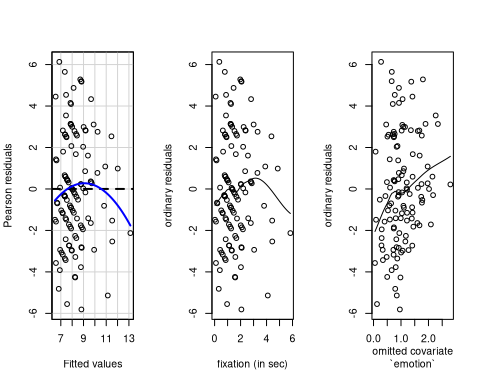
\includegraphics[width=0.7\linewidth]{Statistical-modelling_files/figure-latex/residlowess-1} \end{center}

There is no graphical in our example that the relationship between fixation time and buying intention is nonlinear --- the dip in fitted value and fixation is spurious and is due to the lack of long fixation time, which means the point has high leverage and pulls the smooth to itself.

If we plot the omitted covariate \texttt{emotion}, we see that the local trend is positive and possibly non-zero. This seems to imply that the effect of emotion has not been captured by the model, suggesting that our simple linear regression mean model is overly simple. The extension from simple to multiple linear regression models is straightforward and we can assess the significance of an added variable and test for their significance. In practice, we should use added-variable plots for new variables.

Contrast the lack of residual structure between \texttt{intention} and \texttt{fixation} with the relation between horsepower and fuel consumption in miles per gallon of the \texttt{auto} dataset: we can see a clear nonlinear (potentially quadratic) relationship between distance per gallon and fuel consumption.

\begin{Shaded}
\begin{Highlighting}[]
\NormalTok{url <-}\StringTok{ "https://lbelzile.bitbucket.io/MATH60619A/auto.csv"}
\NormalTok{auto <-}\StringTok{ }\KeywordTok{read.csv}\NormalTok{(url, }\DataTypeTok{header =} \OtherTok{TRUE}\NormalTok{)}
\NormalTok{lmauto <-}\StringTok{ }\KeywordTok{lm}\NormalTok{(mpg }\OperatorTok{~}\StringTok{ }\NormalTok{horsepower, }\DataTypeTok{data =}\NormalTok{ auto)}
\CommentTok{# residual plots (Pearson resid = ordinary resid)}
\NormalTok{car}\OperatorTok{::}\KeywordTok{residualPlots}\NormalTok{(lmauto, }\DataTypeTok{tests =} \OtherTok{FALSE}\NormalTok{)}
\end{Highlighting}
\end{Shaded}

\begin{center}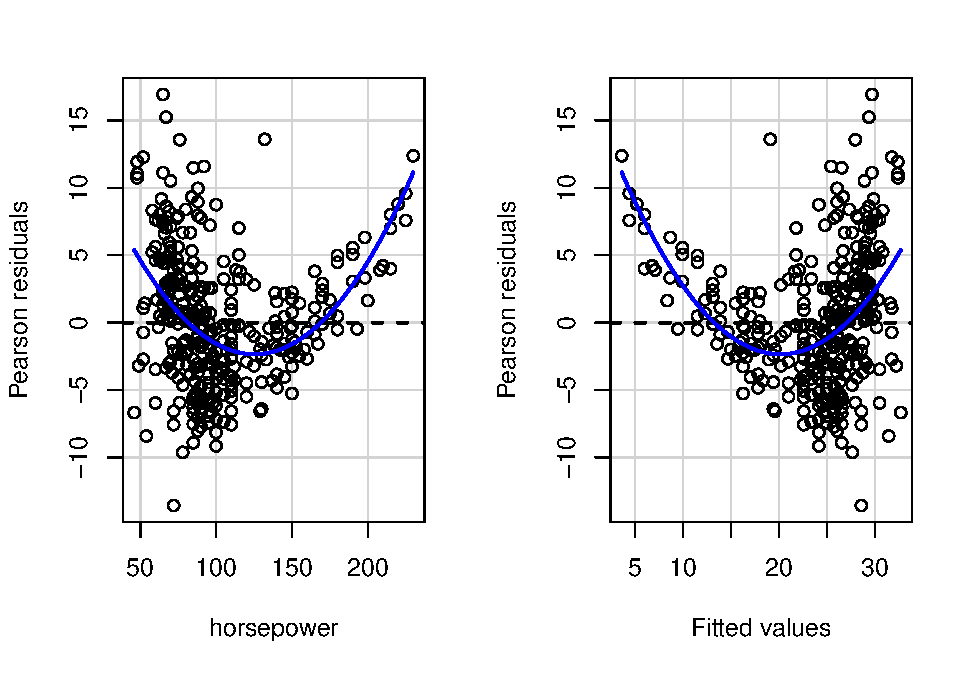
\includegraphics[width=0.7\linewidth]{Statistical-modelling_files/figure-latex/autoplot-1} \end{center}

While \texttt{plot} method for \texttt{lm} objects return plots, the functions in the library \texttt{car} give nicer and often clearer output.

For heteroscedasticity, we can use the absolute jackknife studentized residuals rather than the ordinary residuals: the rationale is that the latter have different variance \(\sigma^2(1-h_i)\), where \(h_i\) is a known constant that depends on \(\mathbf{X}\). The jackknife studentized residuals are thus standardized residuals, whereby each \(e_i\) is divided by an estimate of its standard deviation so that each has the same variance and we can make comparisons. The term jackknife comes from the estimation method. If the \(\varepsilon_i\) are truly normally distributed, then the jackknife studentized residuals should follow a Student with \(n-k-1\) degrees of freedom, where \(k\) is the number of \(\beta\) parameters estimated. If \(n-k\) is large, say larger than 25, we can use the normal distribution for comparison.

\begin{Shaded}
\begin{Highlighting}[]
\KeywordTok{par}\NormalTok{(}\DataTypeTok{mfrow =} \KeywordTok{c}\NormalTok{(}\DecValTok{1}\NormalTok{,}\DecValTok{3}\NormalTok{))}
\CommentTok{# check for heteroscedasticity with jsr}
\KeywordTok{plot}\NormalTok{(}\DecValTok{1}\OperatorTok{:}\KeywordTok{length}\NormalTok{(jsr), }\KeywordTok{abs}\NormalTok{(jsr), }
     \DataTypeTok{xlab=}\StringTok{"observation number"}\NormalTok{, }
     \DataTypeTok{ylab=}\StringTok{"|jackknife studentized residuals|"}\NormalTok{)}
\CommentTok{#a fancy smoother}
\NormalTok{car}\OperatorTok{::}\KeywordTok{gamLine}\NormalTok{(}\DecValTok{1}\OperatorTok{:}\KeywordTok{length}\NormalTok{(jsr), }\KeywordTok{abs}\NormalTok{(jsr), }\DataTypeTok{spread =} \OtherTok{TRUE}\NormalTok{)}
\CommentTok{#density plot}
\NormalTok{car}\OperatorTok{::}\KeywordTok{densityPlot}\NormalTok{(jsr)}
\NormalTok{dfjsr <-}\StringTok{ }\NormalTok{linmod}\OperatorTok{$}\NormalTok{df.residual }\OperatorTok{-}\StringTok{ }\NormalTok{1L}
\CommentTok{#superimpose density of student}
\KeywordTok{curve}\NormalTok{(}\KeywordTok{dt}\NormalTok{(x, }\DataTypeTok{df =}\NormalTok{ dfjsr), }
      \DataTypeTok{from =} \DecValTok{-5}\NormalTok{, }
      \DataTypeTok{to =} \DecValTok{5}\NormalTok{, }
      \DataTypeTok{add =} \OtherTok{TRUE}\NormalTok{,}
      \DataTypeTok{col =} \StringTok{"red"}\NormalTok{)}
\CommentTok{# student q-q plot of jackknife resid}
\NormalTok{car}\OperatorTok{::}\KeywordTok{qqPlot}\NormalTok{(jsr, }
            \DataTypeTok{distribution =} \StringTok{"t"}\NormalTok{, }
            \DataTypeTok{df =}\NormalTok{ dfjsr,}
            \DataTypeTok{ylab =} \StringTok{"jackknife studentized residuals"}\NormalTok{)}
\end{Highlighting}
\end{Shaded}

\begin{center}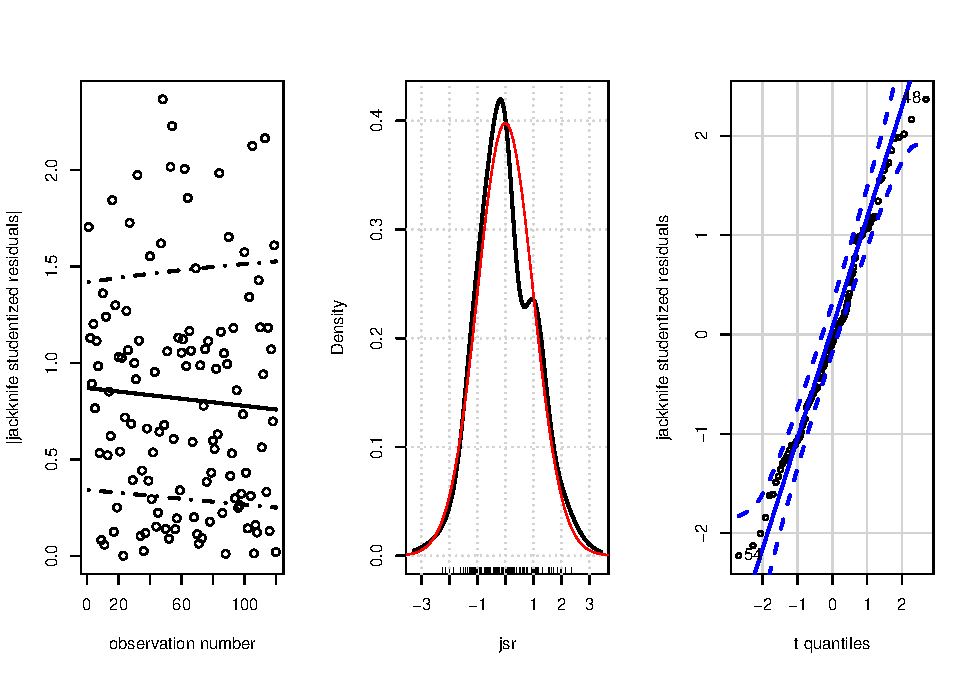
\includegraphics[width=0.7\linewidth]{Statistical-modelling_files/figure-latex/normalitychecks-1} \end{center}

\begin{verbatim}
## [1] 48 54
\end{verbatim}

Here, we see no evidence of heteroscedasticity; the latter is more frequent in multiplicative models, when effects typically increase over time (like growth whose increase is, according to economic theory, exponential). The kernel density estimator (with rugs) and the quantile-quantile plots show that most points are in line with the postulated Student distribution, there is no outlier or extreme value and the residuals are symmetrically distributed around zero.

Interpretation of quantile-quantile plots requires experience; \href{https://stats.stackexchange.com/questions/101274/how-to-interpret-a-qq-plot/101290\#101290}{this post by \emph{Glen\_b} on StackOverflow} nicely summarizes what can be detected (or not) from the Q-Q plot.

\hypertarget{binary-explanatory-variable}{%
\subsection{Binary explanatory variable}\label{binary-explanatory-variable}}

We have seen in class that the two-sample \(t\)-test is a special of linear regression and that we can use the same model. The default parametrization is the so-called \textbf{contrasts}, whereby the intercept \(\beta_0\) correspond to the mean of the baseline, i.e., reference group and \(\beta_1\) is the difference between the two groups. The summary table gives the \(t\)-test for the two-sided test \(\beta_1=0\) with the alternative \(\beta_1 \neq 0\).

For example, compare the output of the following two commands:

\begin{Shaded}
\begin{Highlighting}[]
\KeywordTok{summary}\NormalTok{(}\KeywordTok{lm}\NormalTok{(intention }\OperatorTok{~}\StringTok{ }\NormalTok{sex, }\DataTypeTok{data =}\NormalTok{ intention))}
\end{Highlighting}
\end{Shaded}

\begin{verbatim}
## 
## Call:
## lm(formula = intention ~ sex, data = intention)
## 
## Residuals:
##    Min     1Q Median     3Q    Max 
## -5.919 -2.552  0.081  2.173  5.448 
## 
## Coefficients:
##             Estimate Std. Error t value Pr(>|t|)    
## (Intercept)    7.552      0.376   20.07   <2e-16 ***
## sexwoman       1.368      0.523    2.61     0.01 *  
## ---
## Signif. codes:  0 '***' 0.001 '**' 0.01 '*' 0.05 '.' 0.1 ' ' 1
## 
## Residual standard error: 2.9 on 118 degrees of freedom
## Multiple R-squared:  0.0547, Adjusted R-squared:  0.0467 
## F-statistic: 6.83 on 1 and 118 DF,  p-value: 0.0102
\end{verbatim}

\begin{Shaded}
\begin{Highlighting}[]
\KeywordTok{t.test}\NormalTok{(intention }\OperatorTok{~}\StringTok{ }\NormalTok{sex, }\DataTypeTok{data =}\NormalTok{ intention, }\DataTypeTok{var.equal =} \OtherTok{TRUE}\NormalTok{)}
\end{Highlighting}
\end{Shaded}

\begin{verbatim}
## 
##  Two Sample t-test
## 
## data:  intention by sex
## t = -3, df = 118, p-value = 0.01
## alternative hypothesis: true difference in means is not equal to 0
## 95 percent confidence interval:
##  -2.40 -0.33
## sample estimates:
##   mean in group man mean in group woman 
##                 7.6                 8.9
\end{verbatim}

It turns out that the value of the test statistic and the \(p\)-value for the two-sample \(t\)-test are the same as those of the linear regression for the coefficient \(\beta_1\) corresponding to women. \href{https://lindeloev.github.io/tests-as-linear/}{In fact, many tests we cover can be cast as linear models}. The intercept parameter \(\beta_0\) is the average of men, whereas \(\beta_0+\beta_1\) is the average of women. The advantage of doing a linear regression is that we can quantify the effect of sex while accounting for other potential explanatories.

  \bibliography{book.bib,packages.bib}

\end{document}
